\documentclass[12pt]{article}

\usepackage{fullpage}
\usepackage{breqn}
\usepackage{epsfig}
\usepackage{longtable}
\usepackage{fontenc}
\usepackage{graphicx}
\usepackage{times}
\usepackage{rotating}
\usepackage{psfrag}
\usepackage{graphics}
\usepackage{lscape}
\usepackage{xspace}
\usepackage{hyperref}


\bibliographystyle{input/prsty}

\makeatletter
\renewcommand{\thefootnote}{\fnsymbol{footnote}}
\newcommand{\boldsymbol}[1]{\mbox{\boldmath $#1$}}
\makeatother

\def\totaldays{38~}
\def\productiondays{30~}
\def\overheaddays{8.6~}

\def\QMIN{1.0}
\def\QMAX{1.9}
\def\XMIN{0.80}
\def\XMAX{1.75}
\def\WMIN{0.59}
\def\WMAX{1.09}
\def\Azz{$A_{zz}$}

\def\SPOKES{1}
\def\CONTACT{2}

\def\PZ{50}     % Vector target polarization
\def\PZZ{30}
\def\PF{0.65}   % Packing Factor
\def\DF{0.285}   % Dilution Factor
\def\TARGET{ND$_3$ }
\def\CURRENT{90 } % nanoAmps
\def\LUMI{$1.3\times 10^{35}~\mathrm{cm}^{-2}\mathrm{s}^{-1}$}

\def\be{\begin{eqnarray*}}
\def\ee{\end{eqnarray*}}
\def\bn{\begin{eqnarray}}
\def\en{\end{eqnarray}}
\def\nn{\nonumber}

\def\ks{\vspace{1.1cm}\\}
\def\ls{\vspace{0.1cm}}

\def\n{\large}




%%%%%%%%%%%%%%%

\begin{document}

\pagestyle{empty}
 
\begin{center}
 \LARGE{
  Tensor Asymmetry $A_{zz}$ in the $x>1$ Region
 }
\end{center}
%
\hrule \vspace{.05cm}\hrule
%
\begin{center}
A Proposal to Jefferson Lab PAC 42

\vspace{1.5cm}

\setcounter{footnote}{\SPOKES}
%
{T. Badman,
~~E. Long,\setcounter{footnote}{\SPOKES}
\setcounter{footnote}{\SPOKES}\footnotemark \footnotetext{Spokesperson}
\setcounter{footnote}{\CONTACT}\footnotemark\footnotetext{Contact: \href{mailto:ellie@jlab.org}{ellie@jlab.org}}
~~K. Slifer,\setcounter{footnote}{\SPOKES}\footnotemark
~~P. Solvignon\setcounter{footnote}{\SPOKES}\footnotemark
~~R. Zielinski
}\\
\ls
{\normalsize\it{University of New Hampshire, Durham, NH 03861}}

\vspace{10px}

{~~D. Day,\setcounter{footnote}{\SPOKES}\footnotemark
~~D. Keller,\setcounter{footnote}{\SPOKES}\footnotemark
~~V. Sulkowsky}\\
\ls
{\normalsize\it{University of Virginia, Charlottesville, VA 22903}}

\vspace{10px}

{~~D. Higinbotham\setcounter{footnote}{\SPOKES}\footnotemark}\\
\ls
{\normalsize\it{Thomas Jefferson National Accelerator Facility, Newport News, VA 23606}}

\vspace{10px}

{~~N. Kalantarians}\\
\ls
{\normalsize\it{Hampton University, Hampton, VA 23668}}

\vspace{10px}

{~~M. Sargsian}\\
\ls
{\normalsize\it{Florida International University, Miami, FL 33199}}

\vspace{10px}

{~~M. Strikman}\\
\ls
{\normalsize\it{Pennsylvania State University, University Park, PA 16802}}
\ks
%

\end{center}

%\footnotetext{Co-spokesperson}
%\footnotetext{Contact person}

\setcounter{footnote}{0}


\newpage

\begin{abstract}
  

The tensor-polarized target asymmetry, $A_{zz}$, which is used to extract $b_1$ in the DIS region and is proportional to $T_20$ in the elastic region through the D($e,e'$)X channel, can be used to extract information on the ratio of the S- and D-states in the deuteron wave function. This ratio is currently not well constrained experimentally and is an important quantity to determine for understanding tensor effects such as NN short range correlations.

In the quasi-elastic region, $A_{zz}$ was first calculated in 1988 by Frankfurt and Strikman, using the Hamada-Johnstone and Reid soft-core wave functions \cite{Frankfurt:1988nt}. Recent calculations by {M.~Sargsian} revisit $A_{zz}$ in the $x>1$ range using virtual-nucleon and light-cone methods, which differ by up to a factor of two \cite{MISAK}.

An experimental determination of $A_{zz}$ could be performed utilizing identical equipment identical as the E13-12-011 $b_1$ experiment at three different $Q^2$ values over the course of \productiondays days, with \overheaddays additional days of overhead. The measurements are less sensitive to systematic uncertainties than E13-12-011, such that this experiment could additional be used to understand the in-beam conditions of a tensor polarized target.
\end{abstract}

\newpage

%\section*{Foreword}

%This proposal is an update to PR12-11-110 which was submitted to PAC38.  For convenience, we reproduce the PAC report on the next page.   We provide here an overview of the actions we've taken to address the PAC concerns. Full details are available in the main text.

As suggested by PAC38, we have modified our experimental technique to measure the tensor asymmetry instead of the cross section difference.  This takes the simplified form of the ratio of tensor polarized to unpolarized cross-sections shown in Eq.~\ref{3}.   While this cancels the largest first order effects\footnote{For example, the target magnetic field will be oriented along the beamline during both polarized and unpolarized data taking, which greatly reduces the sensitivity to changes in acceptance in the two configurations.}, special care will be needed to control the sensitivity of the integrated counts in each state to time dependent drifts in detector response, charge measurement and luminosity. 

We have assumed a tensor polarization (P$_{zz}$=\PZZ\%) which is larger than the previous proposal. This assumption is based on the documentation of tensor polarized targets previously discussed in publications, and is supported by the experience of the collaboration's polarized target groups.   This will require incremental development of existing DNP techniques.  We acknowledge that less established methods, such as the `hole-burning' technique recommended by the PAC, hold very good potential to produce significantly higher tensor polarization, but this will require significant R\&D.  We have initiated this process, although from a practical perspective, the funding for this development will likely remain limited until an approved experiment demonstrates the need for these novel tensor polarized targets. 

The $x_B$-coverage has been expanded, although we note that a significantly non-zero value of $b_1$ at any $x_B$ would unambiguously confirm its non-conventional behavior.  Finally, we have engaged several theorists for calculations and to confirm that our interpretation of the relationship between the measured asymmetry and the tensor structure function $b_1$ is valid.



\newpage
\subsection*{PAC38 Report}
{
\noindent
{\bf PR12-11-110} ``The Deuteron Tensor Structure Function b1''

\vspace{0.1cm}
\noindent
{\bf Motivation}: This proposal, a follow-up of LOI-11-003 submitted to PAC37, is dedicated to the measurement of the deuteron tensor structure function $b_1$ by measuring deep inelastic scattering from a tensor polarized deuterium target. All available models predict a small or vanishing value of $b_1$ at low x, however the first pioneering measurement of $b_1$ at HERMES revealed a crossover to an anomalously large negative value, albeit with a relatively large experimental uncertainty. This justifies the intention to make a precise measurement: confirmation that $b_1$ is relatively large may then require an explanation based on more exotic models for the deuteron, such as hidden color due to a 6-quark configuration.

%\vspace{1cm}
\noindent
{\bf Measurement and Feasibility}: The collaboration proposes to carry out this experiment in Hall C, using the polarized UVa/JLab ND$_3$ target, the HMS/SHMS spectrometers and an unpolarized 115 nA electron beam. The tensor structure function $b_1$ is derived from the measurement of the difference between the transversely and longitudinally tensor polarized cross-sections, which is directly proportional to $b_1$ itself. From the measured value of $b_1$ the tensor asymmetry $A_{zz}$ can be calculated, provided the structure function $F_1$ is known. The collaboration proposes to perform the measurement in 28 days of data taking at 11 GeV at the two x values of 0.3 and 0.5, which cover the range in which the HERMES data display the crossover of $b_1$ to large negative values.



%\vspace{1cm}
\noindent
{\bf Issues}: Despite the interesting physics case presented, the PAC has identified several issues with this proposal.
\begin{enumerate}
\item One obvious problem is the theoretical interpretation of the results of this kind of experiments. Following the recommendation of PAC37 the collaboration has partially addressed this question by expanding the discussion of the expected behavior of $b_1(x)$ in various theoretical models. However to draw significant conclusions from this measurement, also given the limited kinematical coverage (see below) chosen, would require further work.
\item The chosen x range, although overlapping with the region in which the HERMES results were obtained, does not seem sufficient to determine $b_1(x)$ in such a way as to unambiguously establish its conventional or exotic behavior. The PAC encourages the collaboration to explore the possibility to carry out the measurement using a large acceptance spectrometer covering a wider x range.
\item The PAC has concerns about the proposed experimental method using the cross section difference between the transversely and longitudinally tensor polarized target configurations. Given a 5-tesla field for this type of target, the effect on the acceptance due to the target field for these configurations can be quite different, and such systematic uncertainties due to the acceptance and other effects may well be larger than the effect that the proponents are trying to measure.
\item The proponents should pursue the tensor asymmetry measurement technique. Currently, the proposed target has a rather low tensor polarization ($\sim$10\%). It is crucial and important to pursue more vigorously techniques such as the RF ``hole’’ burning technique to improve the tensor polarization of the target.
%}
\end{enumerate}
}




\clearpage


\tableofcontents


\pagestyle{plain}

\clearpage

%\section{Quotes (To be removed)}
%``The most direct evidence for tensor correlations in nuclei comes from measurements of the deuteron structure functions and tensor polarization by elastic electron scattering~\cite{Gilman:2001yh}. In essence, these measurements have mapped out the Fourier transforms of the charge densitites of the deuteron in states with spin projections $\pm1$ and 0, showing that they are very different."~-R. Schiavilla, et al.~\cite{Schiavilla:2006xx}


``The cross section for the double scattering process can be written as~\cite{Arnold:1979cg}
\begin{dmath}
	\frac{d\sigma}{d\Omega d\Omega_2} = \left. \frac{d\sigma}{d\Omega d\Omega_2}\right|_0 \left[1 + \frac{3}{2}hp_xA_y\sin{\phi_2} + \frac{1}{\sqrt{2}}t_{20}A_{zz} - \frac{2}{\sqrt{3}}t_{21}A_{xz}\cos{\phi_2}+\frac{1}{\sqrt{3}}t_{22}\left( A_{xx} - A_{yy} \right) \cos{2\phi_2}  \right]
\end{dmath}
where $h=\pm 1/2$ is the polarization of the incoming electron beam, $\phi_2$ the angle between the two sattering planes (defined in the same way as the $\phi$ shown in figure 24) and $A_y$ and the $A_{ij}$ are the vector and tensor analysing powers of the second scattering. Although there is a $p_z$ component to the vector polarization, the term is omitted from equation (25) as there is no longitudinal vector analysing power; without spin precession, this term cannot be determined."~-R. Gilman and F. Gross~\cite{Gilman:2001yh}

``Accurate [form factor] measurements require that $Q^2$ be known accurately since $A$ and $B$ vary rapidly with $Q^2$. Energy or angle offsets of a few times $10^{-3}$ could lead to $Q^2$ being off by up to $0.5\%$. For both $A$ and $B$, this leads to offsets that increase with $Q^2$, reaching about 2\% at $Q^2=1\mathrm{~GeV}^2$ and 4\% at $Q^2=6\mathrm{~GeV}^2$."~-R. Gilman and F. Gross~\cite{Gilman:2001yh}

``The body of [$A$] data, aside from the lowest $Q$ Orsay point, suggests the correctness of the Saclay measurements. Theoretical predictions span the range between the two data sets, and do not help to determine which is correct. Thus, a new high-precision experiment in this [higher] $Q^2$ range appears desirable."~-R. Gilman and F. Gross~\cite{Gilman:2001yh}

``We are forced to conclude that these high $Q^2$ [form factor] measurements \emph{cannot be explained by nonrelativistic physics and present very strong evidence for the presence of interaction currents, relativistic effects or possibly new physics}."~-R. Gilman and F. Gross~\cite{Gilman:2001yh}

``It is now known that the tensor part of the one-pion exchange interaction is too strong to be treated pertubatively, and recent work has focused on how to include the singular parts of one-pion exchange in the most effective manner~\cite{Phillips:1999hh,Phillips:1999am,Walzl:2001vb}"~-R. Gilman and F. Gross~\cite{Gilman:2001yh}

``But a principal motivation for using the front-form is that it is a natural choice at very high momentum, where the interactions single out a preferred direction (the beam direction) and the dynamics evolves along the light-front in that direction. The disadvantage is that the generators that contain dynamical quantities ar $H_{-}$ and $J^i$, and this means that angular momentum conservation must be treated as a dynamical constraint."~-R. Gilman and F. Gross~\cite{Gilman:2001yh}

``Calculations based on quark degrees of freedom must confront the fact that the deuteron is at least a six-quark system. Since the six quarks are identical (because of internal symmetries) the system must be antisymmetrized, and it is not clear that the nucleon should retain its identity in the presence of another nucleon."~-R. Gilman and F. Gross~\cite{Gilman:2001yh}

``It is clear that much more work will be needed to clarify the various physics issues, before a convergent scheme is established for treating the e.m. and strong interaction physics properly."~-J.A. Tjon~\cite{Tjon.48218}

``... there is no clearly correct way to isolate the structure of the nucleon from the structure of the bound state. In model calculations these issues can be handled by separating the problem into two regions: at large separations ($R>R_c$) it is assumed that the system separates into two nucleons interacting through one pion exchange, and at small distances ($R<R_c$) the system is assumed to coalesce into a six-quark bag with all the quarks treated on an equal footing."~-R. Gilman and F. Gross~\cite{Gilman:2001yh}

``It turns out that this leading twist pQCD estimate is $10^3-10^4$ times smaller than the measured deuteron form factor, implying large soft contributions to the form factor, in agreement with \cite{Isgur:1988iw,Radyushkin:1990te}, suggesting that pQCD should not be used as an explanation for the form factor. The calculation is extremely complicated and a confirmation, or refutation, is desirable."~-R. Gilman and F. Gross~\cite{Gilman:2001yh}

``From the discussions in section 3.8, it is clearly of interest to extend measurements of $A$ to higher $Q^2$. An $ed$ coincidence experiment is straightforward, but prohibitive timewise with present accelerators. The proposed 12~GeV JLab upgrade allows one to take advantage of the approximate $E^2$ scaling of $\sigma_M$ at constant $Q^2$ and high energy~\cite{Petratos:2002wz}. A large acceptance spectrometer such as MAD would be very helpful. Depending on the details of the upgrade, a one month experiment could provide data to $Q^2$ of 8 GeV$^2$."~-R. Gilman and F. Gross~\cite{Gilman:2001yh}

``Within the context of a more realistic dynamical theory, one can use response function separations and polarization observables to enhance the sensitivity to various model dependent \emph{unobservables}, such as momentum distributions, meson exchange currents and medium modifications. One strong recent interest has been to choose kinematics in which the unobserved nucleon has a large momentum; the plane wave approximation shows that this configuration enhances sensitivity to initial-state short-range correlations (i.e. the wavefunction) and possibly quark effects. A number of these experiments have been carried out at various accelerators, but no experiments at JLab have yet reported the results."~-R. Gilman and F. Gross~\cite{Gilman:2001yh}

``The most precise constraint on these [$I=1$ exchange] currents comes from the $d\rightarrow ^1S_0$ transition, and this part of the trainsition is partly obscured by the poor renergy resolution of the existing high $Q^2$ measurements. A new and improved experiment at JLab with higher resolution would allow the threshold $d\rightarrow ^1S_0$ process to be better extracted, with a better resulting determination of the isovector exchange currents. It is also important to determine whether or not there is a minimum near 1.2 GeV$^2$."~-R. Gilman and F. Gross~\cite{Gilman:2001yh}

``The nucleon-nucleon ($NN$) interaction has strong tensor forces at long and intermediate distances caused by the pion exchange, which emerges large momentum transfer, and also strong central repulsions at short distance caused by the quark dynamics~\cite{Pieper:2001mp,Kamada:2001tv}. It is important to investigate the nuclear structure by treating these characteristics of the $NN$ interaction."~-T. Myo~\cite{Myo:2013dya}

``From those results, only the $^6$Li ground state show the $LS$ coupling structure and this can be related to the $\alpha + d$ clustering in the $T=0$ state. ... The detailed analyses including the excited states are performed in our paper~\cite{Myo:2012pv}."~-T. Myo~\cite{Myo:2013dya}

``SRCs are considered one of the most elusive features of the ground state nuclear wave functions."~-M. Sargsian~\cite{Sargsian:2012gj}

``One of the methods in probing 2N SRCs is studying high $Q^2$ inclusive $A(e,e')X$ scattering at $x>1.4$ in which case virtual photon scatters off the bound nucleon with momenta exceeding $k_F(A)$~\cite{Sargsian:2001ax, Sargsian:2002wc}."~-M. Sargsian~\cite{Sargsian:2012gj}

``Another recent news from SRC studies is the observation of a strong (by factor of 20) dominance of $pn$ relative to $pp$ and $nn$ SRC's in the range of the bound nucleon momenta $k_F<p<600 \mathrm{MeV}/c$\cite{Piasetzky:2006ai,Subedi:2008zz}. This observation of was an indication that at the distances relevant to the above momentum range the NN force is dominated by tensor interaction. This gave a new meaning to the above mentioned ratios:
\begin{equation}
	A_2(A) = \frac{2\cdot \sigma_{eA}}{A\cdot \sigma_{ed}},
\end{equation}
which now represent (up to the SRC center of mass motion effect) the probability of finding 2N SRCs in the nucleus A. The observed strong disbalance of $pn$ and $pp/nn$ SRCs allowed also to suggest new approximate relation for the high momentum distribution of protons and neutrons in the nucleus A\cite{McGauley:2011qc}:
\begin{equation}
	n^A_{p/n}(p) = \frac{1}{2x_{p/n}}a_d(A,y)\cdot n_d(p)
\end{equation}
where $x_{p/n}=\frac{Z}{A}/\frac{A-Z}{A}$ and $y=\left| 1-2x_p\right|$."~-M. Sargsian~\cite{Sargsian:2012gj}


\section{Background and Motivation}
%For decades~\cite{PhysRev.81.165}, it has been known that the nucleon-nucleon potential has a short-range repulsive core, which is responsible for the stability of strongly interacting matter. However, a description of the repulsive core remains largely unconstrained and our understanding of QCD dynamics at short distances ($\leq 0.5\mathrm{~fm}$) largely incomplete~\cite{Sargsian:2014bwa}. 

The deuteron is the simplest composite nuclear system, and in many ways it is as important to understanding bound states in QCD as the hydrogen atom was to understanding bound systems in QED.  Our experimental and theoretical understanding of the deuteron remains unsatisfying. By taking a ratio of cross sections of electron scattering from tensor-polarized and unpolarized deuterons, the S and D-wave states can be disentangled, leading to a fuller understanding of the repulsive nucleon core. A measurement of $A_{zz}$ is dependent on the $\frac{D^2-SD}{S^2+D^2}$ ratio and it's evolution with increasing momentum. Originally calculated by L. Frankfurt and M. Strikman~\cite{Frankfurt:1988nt}, this has recently been revisited by M. Sargsian, who calculated $A_{zz}$ in this region using a light cone approach and a virtual nucleon approach. The calculations vary by up to a factor of 2, and can be experimentally determined at the $3-6\sigma$ level.

%A measurement of $A_{zz}$ will put an experimental constraint on the D-state admixture in models of the deuteron wavefunction.

Due to their small size and simple structure, tensor polarized deuterons are ideal for studying nucleon-nucleon interactions. Tensor polarization enhances the D-state wavefunction, which compresses the deuteron to $\sim0.5\mathrm{~fm}$~\cite{Forest:1996kp} 
%in a toroid as shown in Fig.~\ref{fig:dpol-shape}, 
reveals short-range QCD effects. Understanding the nucleon-nucleon potential of the deuteron is essential for understanding short-range correlations as they are largely dependent on the tensor force~\cite{Arrington:2011xs}. We can resolve the short-range structure of nuclei on the level of nucleon and hadronic constituents by utilizing processes that transfer to the nucleon constituents both energy and momentum larger than the scale of the NN short-range correlations, particularly at $Q^2>1~(\mathrm{GeV}/c)^2$. By measuring $A_{zz}$ over a range of $Q^2$, we can  access the evolution of the tensor state dominance, and thus the expected evolution of short range correlation effects.

Additionally, measuring $A_{zz}$ in the quasi-elastic region will fill a gap in measurements done on tensor polarized deuterium. It is directly proportional to the observable used in the elastic region to measure $T_{20}$, by $A_{zz} \propto T_{20}$. In the deep inelastic region, $A_{zz}$ will soon be measured to extract the tensor structure function $b_1$ by the relation $A_{zz} \propto \frac{b_1}{F_1^D}$. Not only will measuring $A_{zz}$ in the quasi-elastic region provide information necessary for understanding the properties of the deuteron and contribution from the tensor force, but it will be the first experiment to bridge a hole in measurements of electron scattering from tensor-polarized deuterons.


%Jefferson Lab is the ideal place to investigate tensor structure in a deuteron target at intermediate and large $x$.  We describe such a measurement in this proposal.

%\subsection{Deuteron Wavefunction}

%\begin{figure}
%\centering
%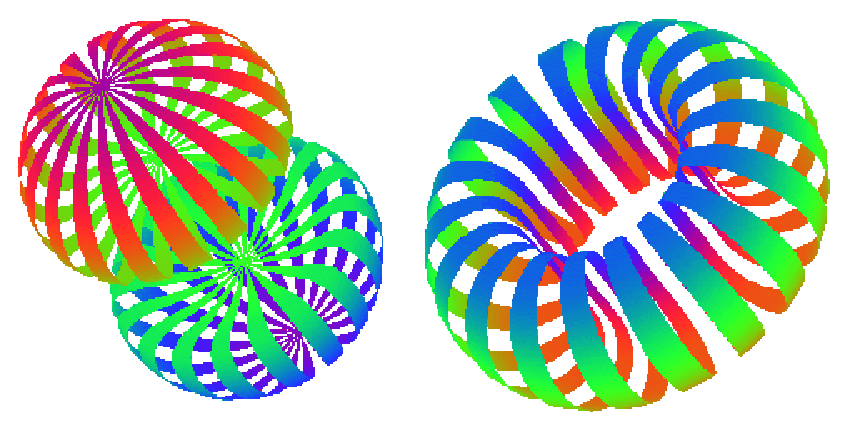
\includegraphics[width=0.5\textwidth]{figs/deuteron_states.eps}
%\caption{\label{fig:dpol-shape}
%Equidensity lines of the deuteron in its two spin projections, $M_J=\pm 1$ and $M_J=0$, respectively. Reproduced from~\cite{Carlson:1997qn,Forest:1996kp}.
%}
%\end{figure}


\subsection{Probing the Deuteron Wavefunction}

It was suggested for some time~\cite{Frankfurt:1981mk} that to resolve the microscopic structure of nuclei one needs to study scattering at sufficiently large momentum transfer and large relative momenta of the produced nucleons. This logic was confirmed~\cite{Arrington:2011xs} by a series of experiments at SLAC~\cite{Frankfurt:1993sp} and JLab~\cite{Arrington:1998ps,Fomin:2011ng} that directly observed short-range correlations (SRC) in a series of nuclei, and established a similar effect of SRC in the deuteron and in heavier nuclei with $pn$ correlations giving the dominant contribution.  Hence, the deuteron serves as a ``hydrogen atom" for the studies of the microscopic short-range structure of the nuclei since it is the simplest nuclei that follows SRC scaling.

To achieve further progress, it is necessary to improve our knowledge of the deuteron wave function at high momenta, and to separate the S and D contributions to the high momentum component of the deuteron. The dominance of the D-wave at large range of the nucleon momenta is expected in a range of the theoretical models as shown in Fig.~\ref{sd-wf}, but experimentally it was probed in a rather indirect way via measurement of $T_{20}$ for the deuteron form factor~\cite{Garcon:2001sz}. Still, the knowledge of S/D ratio for large momenta is rather poor. Indeed, all wavefunctions are constrained by low energy data to reproduce the S/D ratio at small momenta while the overall probability of the D-wave in the deuteron differs by a factor up to 1.5, leading to a large difference of the S/D ratio at large momenta.

The S and D-states are related to the tensor asymmetry $A_{zz}$ by~\cite{Frankfurt:1988nt}
\begin{equation}
	A_{zz} \propto \frac{\frac{1}{2}w^2(k)-u(k)w(k)\sqrt{2}}{u^2(k)+w^2(k)},
\end{equation}
where $u(k)$ is the S-state wave function and $w(k)$ is the D-state wave function. Additionally, measuring $A_{zz}$ at lower $Q^2$ will map out the transition from hadronic to partonic degrees of freedom.

\begin{figure}
\begin{center}
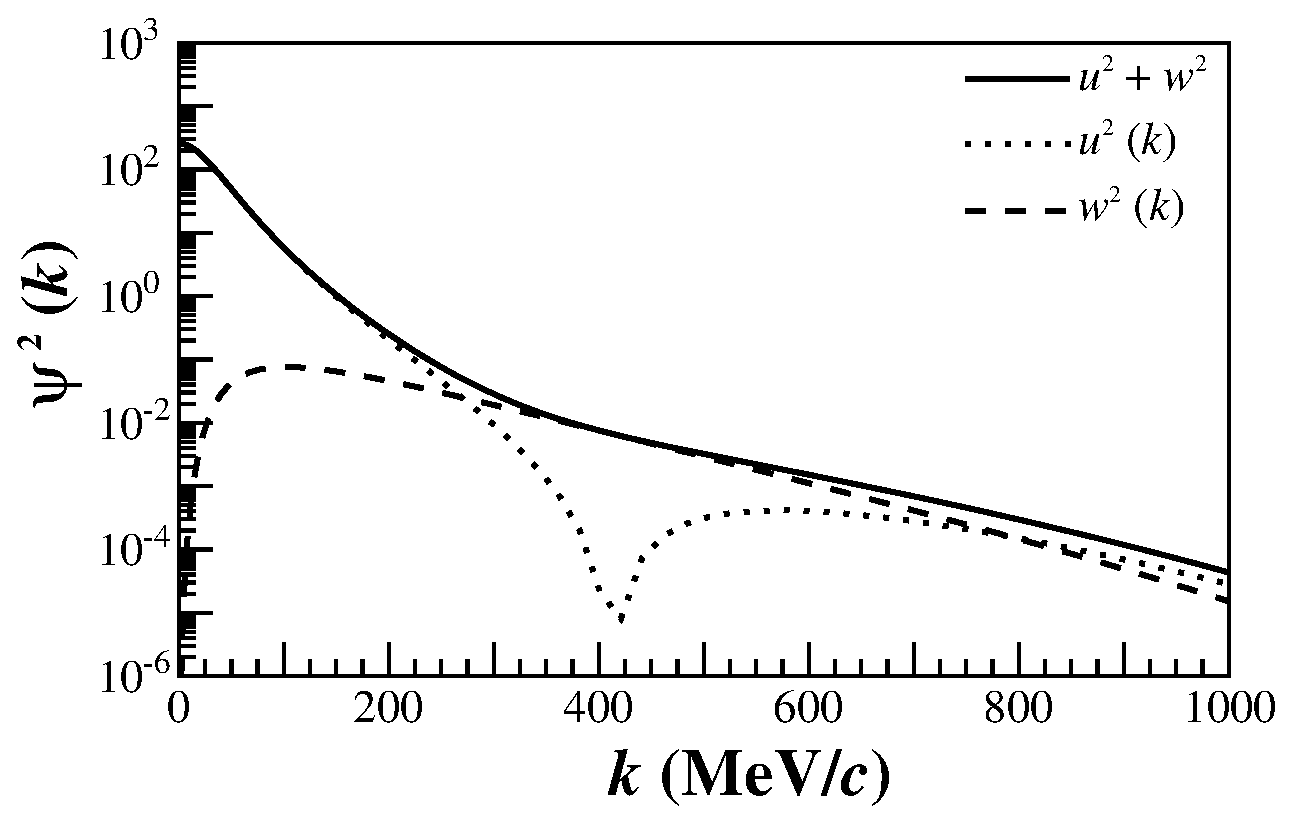
\includegraphics[width=0.55\textwidth]{figs/sd_wf_av18.eps}
\caption{\label{sd-wf} The AV18~\cite{PhysRevC.84.034003} deuteron wave-function, showing the dominance of the D-state (dashed) in comparison to the S-state (dotted) in the full wavefunction (solid) at high momentum ($k>300\mathrm{~Mev}/c$).}
\end{center}
\end{figure}

Ratios of inclusive cross sections at $x>1$ has demonstrated an early onset of the scaling of the ratios when plotted as a function of the light-cone fraction of the struck nucleon momentum.  As a result, the ratios provide a direct measurement of the ratio of the high momentum components in nuclei.  Similarly, one can expect that in the case of scattering from the polarized deuteron we expect the early scaling for the asymmetry when plotted as a function of the minimal struck nucleon momentum or the light cone fraction in the A($e,e’$) case.
It was observed at JLab that the scaling of the ratios is setting in starting at $Q^2 \sim 1 \mathrm{~GeV}^2$ so covering the range of $Q^2$ up to 2~GeV$^2$ will be sufficient to  measure the S/D ratios in an interesting momentum range. 





%For decades~\cite{PhysRev.81.165}, it has been known that the nucleon-nucleon potential has a short-range repulsive core, which is responsible for the stability of strongly interacting matter. However, a description of the repulsive core remains largely unconstrained and our understanding of QCD dynamics at short distances ($\leq 0.5\mathrm{~fm}$) largely incomplete~\cite{Sargsian:2014bwa}. 


It is worth noting here that in addition to comparing predictions for the different wave functions, one expects to be able to distinguish between non-relativistic and light cone quantum mechanic models.  The principal difference between the models is the relation between the spectator momentum and momentum in the wave function in the nonrelativistic model they coincide, while in the light cone model the relation is non-linear starting at $k \sim 250 \mathrm{~MeV}/c$. This difference is most clearly manifested in the scattering off the polarized deuteron due to a strong dependence of the S/D ratio on the nucleon momentum.
%\subsection{Tensor Asymmetry Azz}


The S- and D-states are related to the tensor asymmetry $A_{zz}$ by~\cite{Frankfurt:1988nt}
\begin{equation}
	A_{zz} \propto \frac{\frac{1}{2}w^2(k)-u(k)w(k)\sqrt{2}}{u^2(k)+w^2(k)},
\end{equation}
where $u(k)$ is the S-state wave function and $w(k)$ is the D-state wave function.

For decades~\cite{PhysRev.81.165}, it has been known that the nucleon-nucleon potential has a short-range repulsive core, which is responsible for the stability of strongly interacting matter. However, a description of the repulsive core remains largely unconstrained and our understanding of QCD dynamics at short distances ($\leq 0.5\mathrm{~fm}$) largely incomplete~\cite{Sargsian:2014bwa}. 

Due to their small size~\cite{needed} and simple structure, tensor polarized deuterons are ideal for studying nucleon-nucleon interactions. Tensor polarization enhances the D-state wavefunction, which compresses the deuteron from $\sim?\mathrm{~fm}$ to $\sim0.5\mathrm{~fm}$~\cite{Forest:1996kp} and has been noted to be revealing of short-range QCD effects.


% \subsection{Tensor Structure of the Deuteron}
% %\subsubsection*{Tensor Polarization}
When a  spin 1 system such as the deuteron is subjected to a magnetic field along the z-axis, the
Zeeman interaction gives rise to three magnetic sublevels $I_z = +1,0,-1$ with
population fractions $p_+,p_-, p_0$, respectively.
%\footnote{i.e. $p_+ + p_- +p_0=1$.}.
These populations are described by
both a vector  polarization,
%
\begin{eqnarray}
\nonumber
P_z &=&\langle I_z/I\rangle \\
    &=&(p_+ - p_0) + (p_0-p_+) = p_+ - p_-
\end{eqnarray}
and a tensor polarization~\cite{Meyer:1985dta}:
\begin{eqnarray}
\nonumber
P_{zz} &=& \langle 3 I_z^2 - I(I+1)\rangle/I^2   \\
&=&(p_+ - p_0) - (p_0-p_-) = 1 - 3 p_0
\end{eqnarray}
%
which are subject to the overall normalization $p_+ + p_- + p_0 = 1$.

Fig.~\ref{fig:deuteron} graphically demonstrates the dependence of the two nucleon distribution on the spin projection.  If the two nucleons are in a relative $m=0$ state, the surface of constant density is toroidal, while if they are in the $m=\pm 1$ state, the surface has a dumbbell shape.

\begin{figure}
\centering
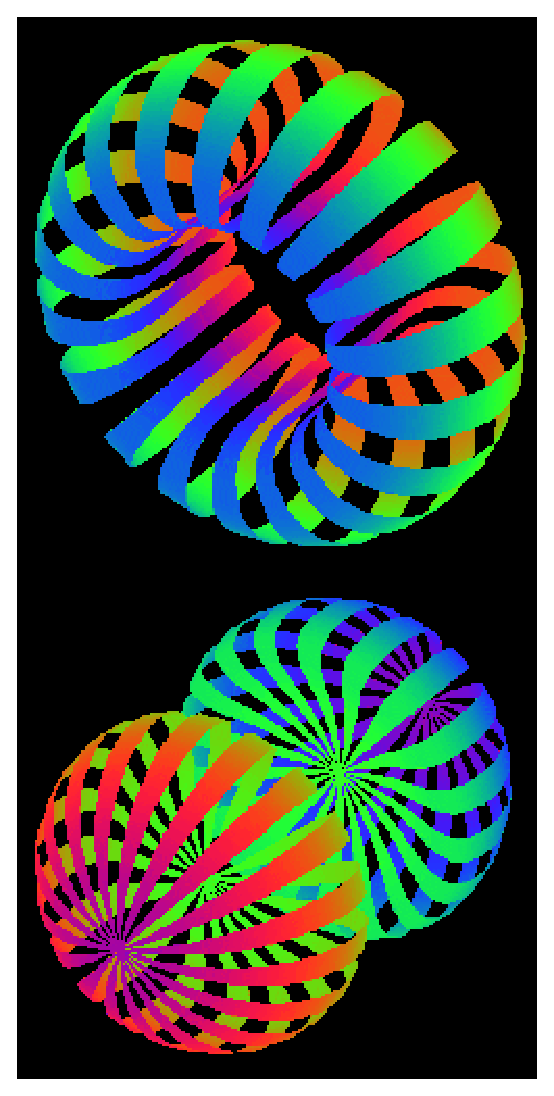
\includegraphics[width=0.3\textwidth,angle=90]{figs/pic-v10-st16-1.eps}
\caption{\label{fig:deuteron}
Nucleon densities of the deuteron in its two spin projections, $I_z=0$ and $I_z=\pm 1$, respectively.
{\it Reproduced from~\cite{Carlson:1997qn,Forest:1996kp}}.
}
\end{figure}

In the case of deuteron spins in thermal equilibrium with the solid lattice, and neglecting the small quadrupole interaction~\cite{Meyer:1985dta}, the tensor polarization is related to  the vector polarization via:
\begin{eqnarray}
\label{TENSORVECTOR}
P_{zz}= 2 - \sqrt{4-3 P_z^2}
\end{eqnarray}
The maximum absolute value of $P_{zz}=-2$  occurs only for vanishing populations in the $m=\pm 1$ states.
If, on the other hand, only the $m=1$ or $m=-1$ state are occupied, the vector polarization reaches its maximum value of $+1$, and $P_{zz}=+1$.  

% \subsection{Quasi-Elastic and $x>1$ Scattering from Spin-1 Targets}
% %In this case, the familiar structure functions  $F_1$, $F_2$, $g_1$, and $g_2$ which describe
%inclusive scattering of electrons from spin-1/2 targets, must be supplemented for a spin-1 system
%by four additional structure functions : $b_1$, $b_2$, $b_3$, and $\Delta$.
%
%
%The tensor structure function $b_1$, ( which is leading-twist like  $F_1$ and $g_1$), is quite
%interesting, in that it presents a simple gauge of nuclear effects: $b_1$ would vanish if the
%deuteron was simply a proton and neutron in a relative S state.
%
%Nuclear effects/EMC effect
%%When spin physics joins naturally the nuclear effects area and model independent
%%nuclear effects extraction compared to polarized EMC effect.
%
%Exotic components.
%
%The Hermes collaboration  made a first measurement~\cite{Airapetian:2005cb} of
%$b_1$ and found significantly non-zero results.
%Beyond providing insight into nuclear structure, this has the potential to impact $g_1^n$ and
%$g_2^n$ extractions, where $b_1$ has traditionally been ignored when the neutron is extracted
%from deuteron data.
%

Four independent  helicity amplitudes are
sufficient to describe virtual Compton scattering from a spin-1/2 target, after requiring parity
and time reversal invariance.  This number doubles  for
a spin-1 target, as the spin can be in three states (+, 0, -). 
This gives rise to a tensor structure which was first discussed for the deuteron for the real photon case
by Pais~\cite{Pais:1967zz}, %in 1967 
and later in the virtual photon case, by Frankfurt and
Strikman~\cite{Frankfurt:1983qs}. %In 1988, 
Hoodbhoy, Jaffe and Manohar~\cite{Hoodbhoy:1988am}
introduced the notation which we now follow, whereby the tensor structure is described
by the four functions $b_1$, $b_2$, $b_3$ and $b_4$.
To summarize, the hadronic tensor can be decomposed as:
%
\begin{eqnarray}
W_{\mu\nu} &=& - F_1 g_{\mu\nu} + F_2 \frac{P_{\mu} P{\nu}}{\nu} \nonumber \\
          & & - b_1 r_{\mu\nu} + \frac{1}{6} b_2 (s_{\mu\nu} + t_{\mu\nu} + u_{\mu\nu}) \nonumber \\
          & & + \frac{1}{2} b_3 (s_{\mu\nu} - u_{\mu\nu}) + \frac{1}{2} b_4 (s_{\mu\nu} - t_{\mu\nu}) \nonumber \\
          & & + i \frac{g_1}{\nu} \epsilon_{\mu\nu\lambda\sigma} q^{\lambda} s^{\sigma} 
              + i \frac{g_2}{\nu^2} \epsilon_{\mu\nu\lambda\sigma} q^{\lambda} (p \cdot qs^{\sigma}  
              - s \cdot qp^{\sigma})
\label{had-tensor}
\end{eqnarray}
%
where the purely kinematic expressions  $r_{\mu\nu}$, $s_{\mu\nu}$, $t_{\mu\nu}$ and $u_{\mu\nu}$ can be 
found in~\cite{Hoodbhoy:1988am}. The terms are all proportional to the 
polarization of the target $E$. The spin-1 structure functions $F_1$, $F_2$, $g_1$ and 
$g_2$ have the same expressions and are measured the same way as for a spin-1/2 
target. The spin-dependent structure functions $b_1$, $b_2$, $b_3$, $b_4$ are 
symmetric under $\mu\leftrightarrow\nu$ and $E\leftrightarrow E^*$ and therefore can 
be isolated from $F_1$ and $g_1$ by unpolarized beam scattering from a polarized 
spin-1 target.


%\subsubsection{Existing Data}
% \label{B1DATASECTION}
%\begin{figure}
%\begin{center}
%\includegraphics[angle=0,width=0.45\textwidth]{figs/azzfinal.eps}
%
%\includegraphics[angle=0,width=0.47\textwidth]{figs/b1final.eps}
%\caption{\label{HERMES_AZZ} {\bf Top:} HERMES measurement of the inclusive tensor asymmetry A$_{zz}$ of the deuteron.  
%{\bf Bottom:} HERMES measurement of the inclusive tensor structure function b$_1^d$ and the average $Q^2$ for each x-bin.  The error bands displays the total systematic uncertainty.
%{\it Reproduced from~\cite{Riedl:2005jq}.}}
%\end{center}\end{figure}

\begin{figure}
\begin{center}
\includegraphics[angle=0,width=0.45\textwidth]{figs/1.eps}
\hspace{0.5cm}
\includegraphics[angle=0,width=0.45\textwidth]{figs/2.eps}
\vspace{3cm}

\includegraphics[angle=0,width=0.45\textwidth]{figs/3.eps}
\caption{\label{HERMES_AZZ} {\bf Top}: HERMES~\cite{Riedl:2005jq} measurement of the inclusive tensor asymmetry A$_{zz}(x)$ and $xb_1(x)$ of the deuteron. {\bf Bottom} : The tensor structure function $b_1(x)$ without $x$-weighting, which reveals a steep rise as $x\to 0$. 
}
\end{center}\end{figure}

%\begin{figure}
%\begin{center}
%\includegraphics[angle=0,width=0.47\textwidth]{figs/2.eps}
%\caption{\label{HERMES_AZZ2} 
%HERMES~\cite{Riedl:2005jq} measurement of the inclusive tensor structure function b$_1^d$.  
%}
%\end{center}\end{figure}



%\begin{figure}
%\begin{center}
%\includegraphics[angle=0,width=4.in]{figs/azzfinal.eps}
%\caption{\label{HERMES_AZZ} HERMES measurement of the inclusive tensor asymmetry A$_{zz}$ of the deuteron.
%The error band displays the total systematic uncertainty.
%{\it Reproduced from~\cite{Riedl:2005jq}.}}
%\end{center}\end{figure}

%\begin{figure}
%\begin{center}
%\includegraphics[angle=0,width=4.1in]{figs/b1final.eps}
%\caption{\label{HERMES_B1D} HERMES measurement of the inclusive tensor structure function b$_1^d$ and the average $Q^2$ for each x-bin.  The error band displays the total systematic uncertainty.
%{\it Reproduced from~\cite{Riedl:2005jq}.}}
%\end{center}\end{figure}


\begin{figure}
\begin{center}
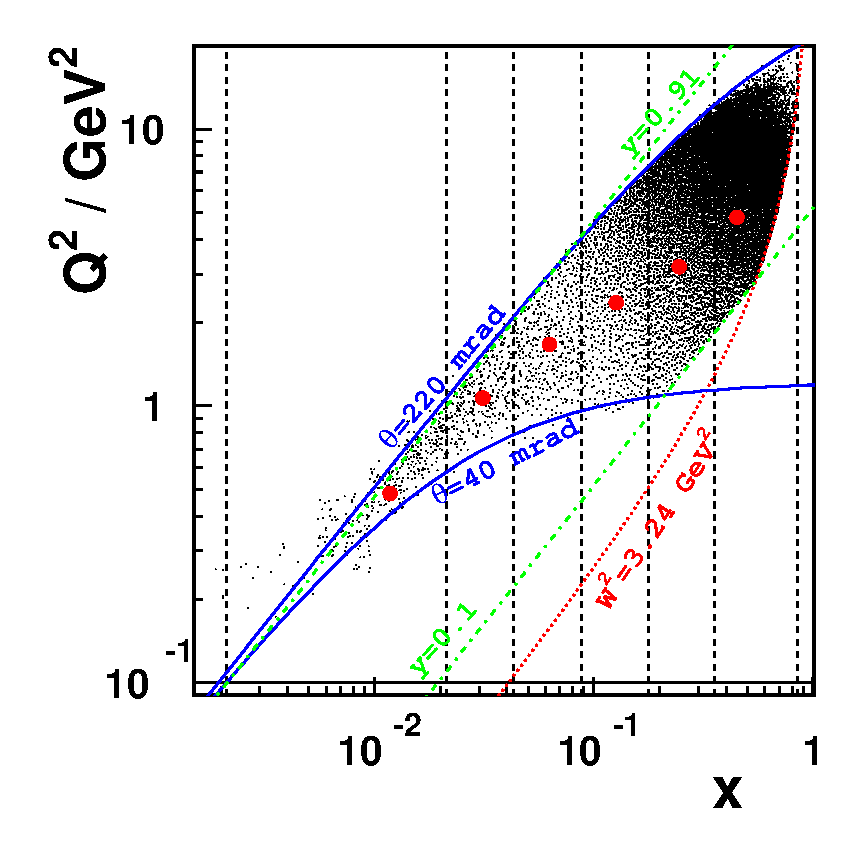
\includegraphics[angle=0,width=0.45\textwidth]{figs/kineplane.eps}
\caption{\label{HERMES_KIN} Kinematic coverage of the HERMES measurement.  The dashed vertical lines indicate the borders
of the bins in x, the dots their centers of gravity. The solid curves
indicate the
vertical acceptance of the spectrometer, defined by its aperture.
In addition, the
kinematic cuts imposed on the variables Q$^2$, y
and W$^2$ are shown. 
%The W$^2$ cut suppresses the nuclear resonance region.
{\it Reproduced from~\cite{Riedl:2005jq}.}}
\end{center}\end{figure}


The HERMES collaboration  made the first measurement~\cite{Riedl:2005jq,Airapetian:2005cb} of
$b_1$ in 2005.
The experiment explored the low $x$ region of $0.001<x<0.45$ for  $0.5<Q^2<5$ GeV$^2$.  
An atomic beam source was used to generate a deuterium gas target with high tensor polarization.  
The HERA storage ring provided 27.6 GeV positrons incident on the internal gas target.

As displayed in Fig.~\ref{HERMES_AZZ}, the tensor asymmetry A$_{zz}$  was found to be 
non-zero at about the  two sigma level, with an apparent zero crossing around $x=0.3$. %  for $x < 0.1$.  
%
The tensor structure function $b_1$ exhibits a steep rise as $x\to 0$, which is qualitatively
in agreement with the predictions of coherent double-scattering models. See for example Ref.~\cite{Edelmann:1997ik}.  The authors of Ref.~\cite{Airapetian:2005cb} interpret the rapid rise at low $x$ in terms of the same mechanism that leads to nuclear shadowing in unpolarized scattering, i.e. double scattering of the lepton, first from the proton, then from the neutron, with sensitivity to the spatial alignment of the two nucleons.
%The Close-Kumano integral (Eq.~\ref{cksum}) was evaluated and found to be:
%\begin{eqnarray}
%\int_{0.0002}^{0.85} b_1(x) dx = 0.0105 \pm 0.0034 \pm 0.0035
%\end{eqnarray}
%which result possibly indicates a breaking of the Close-Kumano sum rule, and consequently a 
%tensor-polarized quark sea.
%%
%%

As is often the case with a pioneer measurement, the precision of the results leaves some
room for ambiguity.  Despite the surprisingly large magnitude and interesting trend of the data, 
all points are roughly within two sigma from zero, which calls for a higher precision measurement.
Another issue is that some of the HERMES momentum transfer values are low 
(see Fig.~\ref{HERMES_KIN}), so that quark structure functions may not be the correct language. 
The $Q^2$ variation in each $x$-bin is also quite wide ($\approx$10 GeV$^2$ for $x\sim 0.3$), which complicates
the interpretation of this data, since  several models predict significant $Q^2$-dependence of
 $b_1$. See for example Fig.~\ref{xb1_pred}.



%\begin{figure}\begin{center}
%\includegraphics[angle=0,width=3.1in]{figs/b1g1.eps}
%\caption{\label{}\footnotesize
%{\it Reproduced from~\cite{Riedl:2005jq}.}}
%\end{center}\end{figure}

%\begin{figure}\begin{center}
%\includegraphics[angle=0,width=3.1in]{figs/b1g1overf1.eps}
%caption{\label{}\footnotesize
%{\it Reproduced from~\cite{Riedl:2005jq}.}}
%\end{center}\end{figure}

%\begin{figure}\begin{center}
%\includegraphics[angle=0,width=3.1in]{figs/b2theo.eps}
%\caption{\label{}\footnotesize
%{\it Reproduced from~\cite{Riedl:2005jq}.}}
%\end{center}\end{figure}


%%%%%%%%%%%%%
%%%%%%%%%%%%%
\subsubsection{Interpretation in the Operator Product Expansion}
%
In the Operator Product Expansion (OPE) framework, the leading operators 
$O_V^{\mu_1...\mu_n}$ and $O_A^{\mu_1...\mu_n}$ in the expansion are twist two. For a 
spin-1 target, the matrix elements of the time-ordered product of two currents 
$T_{\mu\nu}$ have the following expressions:
%
\begin{eqnarray}
<p,E|O_V^{\mu_1...\mu_n}|p,E>&=&S[a_np^{\mu_1}...p^{\mu_n}+d_n(E^{*\mu_1}E^{\mu_2}-\frac{1}{3}p^{\mu_1}
p^{\mu_2})p^{\mu_3}...p^{\mu_n}], \nonumber \\
<p,E|O_A^{\mu_1...\mu_n}|p,E>&=&S[r_n\epsilon^{\lambda\sigma\tau\mu_1}E_{\lambda}^*E_{\sigma}p_{\tau}
p^{\mu_2}...p^{\mu_n}]
\label{matrix-elt}
\end{eqnarray}
%
The non-zero value of $b_1$ arises from the fact that, in a spin-1 target, the 
$\frac{1}{3}p^{\mu_1}p^{\mu_2}$ term doesn't cancel the tensor structure $E^{*\mu_1}E^{\mu_2}$. 
The coefficient $d_n$ can be extracted from the comparison of $T_{\mu\nu}$ expansion 
and the spin-1 target hadronic tensor Eq.~\ref{had-tensor} as follows:
%
\begin{eqnarray}
b_1(\omega)&=&\sum_{n=2,4,...}^\infty 2 C_n^{(1)} d_n \omega^n, \nonumber \\
b_2(\omega)&=&\sum_{n=2,4,...}^\infty 4 C_n^{(2)} d_n \omega^{n-1},
\end{eqnarray}
%
for $1 \le |\omega| \le \infty$ (where $\omega = 1/x$). A Callan-Gross-type relation 
exists for the two leading order tensor structure functions:
%
\begin{eqnarray}
 2 x b_1 = b_2
\label{callan-gross}
\end{eqnarray}
%
valid at lowest order of QCD, where $C_n^{(1)} = C_n^{(2)}$.
At higher orders, Eq.~\ref{callan-gross} is violated.

Sum rules can be 
extracted from the moments of the tensor structure functions:
%
\begin{eqnarray}
\int_0^1 x^{n-1}~b_1(x)~dx &=& \frac{1}{2}~C_n^{(1)}~d_n, \nonumber \\
\int_0^1 x^{n-2}~b_2(x)~dx &=& C_n^{(2)}~d_n,
\label{sr}
\end{eqnarray}
%
where n is even. 

The OPE formalism is based on QCD and is target-independent. However, a target dependence 
is generated by Eq.~\ref{matrix-elt}, and spin-1 structure functions are subject to 
the same QCD corrections and their moments have the same anomalous dimensions as for 
a spin-1/2 target. In addition, the tensor structure functions should exhibit the same 
scaling behavior as $F_1$ and $F_2$, since they are generated from the same matrix 
element $O_V^{\mu_1...\mu_n}$.

We focus in this document on the leading twist structure function $b_1$.  A Callan-Gross type relation allows access to $b_2$ once $b_1$ is determined, and $b_3$ and $b_4$ do not contribute at leading twist.
%%%%%%%%
%%%%%%%%
\subsubsection{Interpretation in the Parton Model}
%
In the infinite momentum frame\footnote{All spins and
momenta are along the $z$-axis.} of the parton model, 
the scattering of the virtual photon from a free quark 
with spin up (or down), which carries a momentum fraction $x$ of the spin-$m$ hadron, can be 
expressed through the hadronic tensor $W_{\mu\nu}^{(m)}$:
%
\begin{eqnarray}
W_{\mu\nu}^{(1)} = \Bigg(- \frac{1}{2} g_{\mu\nu} + \frac{x}{\nu} P_{\mu}P{\nu}\Bigg) 
                               \Big(q^1_{\uparrow}(x) + q^1_{\downarrow}(x)\Big) \nonumber
                    + \frac{i \epsilon_{\mu\nu\lambda\sigma} q^{\lambda} s^{\sigma}}{2 \nu} 
                               \Big(q^1_{\uparrow}(x) - q^1_{\downarrow}(x)\Big),
\label{had-tensor-1}
\end{eqnarray}
%
for a target of spin projection equal to 1 along the $z$-direction, and:
%
\begin{eqnarray}
W_{\mu\nu}^{(0)} = \Bigg(- \frac{1}{2} g_{\mu\nu} + \frac{x}{\nu} P_{\mu}P{\nu}\Bigg) 
                               2 q^0_{\uparrow}(x) 
\label{had-tensor-0}
\end{eqnarray}
%
for a target of spin projection equal to zero along the $z$-direction. The tensor 
structure functions $b_1$ and $b_2$ can be expressed from the comparison of 
$W_{\mu\nu}^{(1)} - W_{\mu\nu}^{(0)}$ with Eq.~\ref{had-tensor} as follows:
%
\begin{eqnarray}
b_1(x) &=& \frac{1}{2} \Big( 2 q^0_{\uparrow}(x) - q^1_{\uparrow}(x) - q^1_{\downarrow}(x) \Big) \\
b_2(x) &=& 2 x b_1(x)
\label{TSF-parton}
\end{eqnarray}
%
where $q^m_{\uparrow}$ ($q^m_{\downarrow}$)  represents the probability to find a quark with momentum fraction $x$ and spin up (down) in a hadron which is in helicity state $m$.
%For example, $q^1_{\uparrow}(x)$ is the probability to find a quark with spin up and momentum fraction $x$ in a deuteron that is in state $m=1$. 
%
The tensor structure function $b_1$ depends only on the spin-averaged parton distributions\footnote{since, by parity, $q^m_{\uparrow}= q^m_{\downarrow}$} 
\begin{eqnarray*}
q^1(x) &=& q^1_{\uparrow}(x) + q^1_{\downarrow}(x)\\ 
q^0(x) &=& q^0_{\uparrow}(x) + q^0_{\downarrow}(x) 
= 2 q^0_{\uparrow}(x)
\end{eqnarray*}
so it can be expressed as:
\begin{eqnarray}
b_1(x) = \frac{q^0(x) - q^1(x)}{2}
\end{eqnarray}

Explicitly, $b_1$ measures the difference
in partonic constituency in an $|m|$=1 target and an $m$=0 target. 
 From this we see that while $b_1$ is defined in terms of quark distributions, it interestingly depends also on the spin state of the nucleus as a whole.

%The three leading twist structure functions are $F_1$, $g_1$ and $b_1$.
%The tensor structure function $b_1$, which is leading-twist like  $F_1$ and 
%$g_1$, is quite interesting, in that it presents a simple gauge of nuclear 
%effects: $b_1$ would vanish if the deuteron was simply a proton and neutron in 
%a relative S state.
%
%
%%The Hermes collaboration  made a first measurement~\cite{Airapetian:2005cb} of 
%$b_1$ and found significantly non-zero results.  Beyond providing insight into
%nuclear structure, this has the potential to impact $g_1^n$ and $g_2^n$ extractions, 
%where $b_1$ has traditionally been ignored when the neutron is extracted from 
%deuteron data.








% \subsection{The Tensor Asymmetry \Azz}
%\label{PREDB1X}
%   %%
The leading twist tensor structure function $b_1$ quantifies effects not present in 
the case of spin-1/2 hadrons. However, tensor effects only
exist in nuclear targets, so the study of $b_1$ serves as a very interesting bridge between nucleon and nuclear physics.
On the one hand, deep inelastic scattering (DIS), clearly probes partonic degrees of freedom, i.e. quarks, but on the 
other hand, $b_1$ depends solely on the deuteron (nuclear) spin state as seen in Eq.~\ref{TSF-parton}. We discuss now several predictions for the $x$ dependence of $b_1$.

%A measurement of $b_1$ would allow us to take 
%a deeper look at the nucleus internal dynamics, since $b_1$ should be zero if the 
%nucleus is made up of spin-1/2 constituents at rest, or in a relative $s$-wave. 
%Therefore a non-negligible value of $b_1$ can be understood in terms of the deviation 
%of a nucleus from a simple bound state of protons and neutrons, 

%
\subsubsection{Conventional Nuclear Effects}
%\subsubsection*{Hoodbhoy, Jaffe and Manohar}
In Ref.~\cite{Hoodbhoy:1988am}, the authors note that $b_1(x)$ is small and calculable for
a weakly bound system like the deuteron, and that its measurement would provide a clear signature 
for exotic components in a spin one nucleus.  In effect, $b_1(x)$ measures the extent to which a target nucleus deviates from a trivial bound state of protons and neutrons.
The authors evaluate the value of $b_1$ in three conventional scenarios for the deuteron
constituents and their dynamics:
\begin{enumerate}
 \item[I.] If the deuteron is composed of two spin-1/2 non-interacting nucleons at rest,
then the eight helicity amplitudes characteristic of a spin-1 target are 
expressed in terms of the four helicity amplitudes of each spin-1/2 nucleons, and 
therefore the total number of independent amplitudes is reduced from eight to four. All structure 
functions of the deuteron are then the simple sum of the structure functions of the two 
nucleons, and the tensor structure functions vanish: $b_1 = b_2 
= b_3 = b_4 = 0$. 
 \item[II.] If instead, the deuteron is composed of two spin-1/2 nucleons moving non-relativistically 
in a central potential, then the target motion modifies the helicity amplitudes. Using
the convolution formalism, it was found that the contribution of these moving nucleons
to $b_1$ is small and is dominated by the lower component of the nucleon's Dirac
wave function.
 \item[III.] In the final scenario considered, the deuteron contains a $D$-state admixture. Because the proton and the neutron
are moving in opposite directions, an additional term due to the $S-D$ interference 
appears in the convolution procedure. This extra contribution to $b_1$ is predicted
to be even smaller than in the previous case.
\end{enumerate}

All three scenarios predict a small or vanishing $b_1$, leading the authors to predict that
$b_1\approx 0$ for the deuteron. 

As an interesting counter example for which 
$b_1$ could be significant, the authors consider a model of a massless relativistic
quark with $j=3/2$ moving in a central potential.  In this calculation, a meson in the $j=1$ state is formed from the coupling of a $P_{3/2}$
massless quark with a spin-1/2 spectator.  This crude model predicts that
$b_1(x)$ exhibits large negative values peaked around $x=0.5$~\cite{Hoodbhoy:1988am}.  
Curiously, this behavior is possibly mirrored by the existing HERMES data (see Fig.~\ref{xb1_pred}), but there is only a single data point with large uncertainty in this region.


\begin{figure}
\begin{center}
%\includegraphics[width=0.40\textwidth]{figs/bora_jaffe_fig3.eps}
%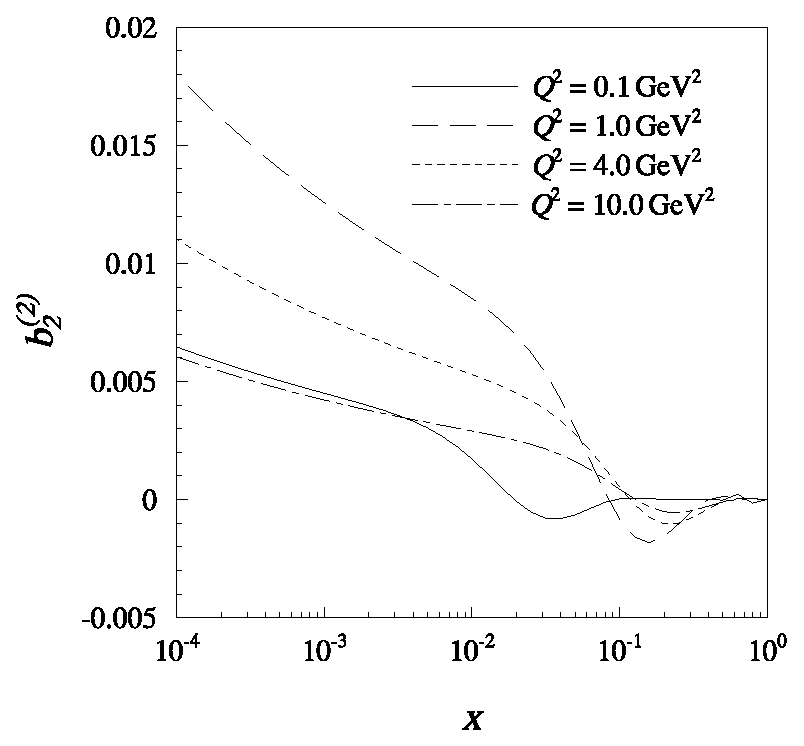
\includegraphics[width=0.3725\textwidth]{figs/bx.eps}
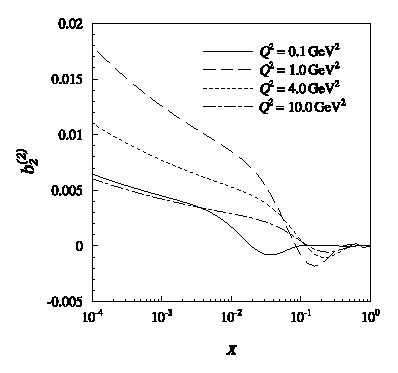
\includegraphics[width=0.3725\textwidth]{newfigs/ellie/figure-4a.eps}
\hspace{0.3cm}
\includegraphics[width=0.45\textwidth]{figs/xb1_mstw_newmiller.eps}
\caption{\label{xb1_pred} Theoretical predictions. {\bf Left plot:} Double-scattering 
contribution to $b_2(x,Q^2)$ as a  function of $x$~\cite{Bora:1997pi}.  Note the strong $Q^2$ dependence at low x.
%($b_2 = b_2^{(1)}+b_2^{(2)}$). 
{\bf Right plot:} HERMES results~\cite{Airapetian:2005cb} compared to calculations 
from S.~Kumano~\cite{Kumano:2010vz} and from the one-pion exchange effects of 
G. Miller~\cite{Miller:1989nc,Miller_tmp}.}
\end{center}
\end{figure}

\begin{figure}
\begin{center}
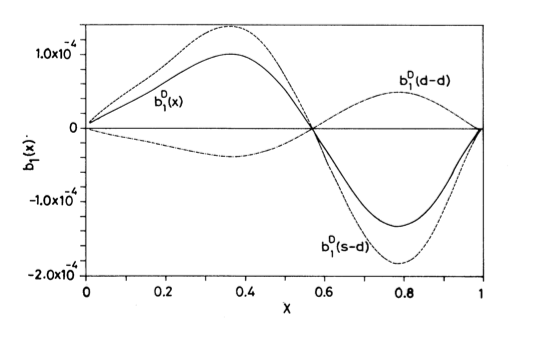
\includegraphics[width=0.45\textwidth]{figs/khan_pervez.eps}
\caption{\label{KHAN} Prediction for b$_1^D(x)$ (solid curve) from Ref.~\cite{Khan:1991qk}, the S-D contribution to b$_1^D(x)$ (dashed curve), and the D-D contribution to b$_1^D(x)$ (dot-dashed curve).  Note the vertical scale which would make the curve mostly indiscernible from zero in Fig.~\ref{xb1_pred} (right). {\it Reproduced from Ref.~\cite{Khan:1991qk}}.
}
\end{center}
\end{figure}
\subsubsection{Nuclear Pions}
In 1988, Miller also examined the tensor structure function $b_1$~\cite{Miller:1989nc}.
The basic mechanism is that the virtual photon hits an exchanged pion  which
is responsible for the binding of the deuteron. 
%The calculation depends on the choice of pion structure function which carries uncertainty. 
In this early calculation, the convention used by Miller for $b_1$ was different from that
used in the HERMES results and in Ref.~\cite{Kumano:2010vz}. A recent update to this  
calculation~\cite{Miller_tmp}, which uses a consistent convention and the pion structure
function from~\cite{Sutton:1991ay}, is shown in Fig.~\ref{xb1_pred}. The spread of the curve originates from the 
parameter $A_s=(.9 \pm 0.3)$ which governs the strength of the sea in the pion. 
Miller's calculation, similar to other `non-exotic' models, is unable to reproduce the trend of the HERMES data, and predicts very small values of $b_1(x)$ at intermediate and large $x$.
%These 
%numbers are all in qualitative agreement with the existing HERMES~\cite{Airapetian:2005cb} data, given their large error bars.
%Coherent-double scattering is expected to contribute also, but is not included in the Miller calculation. 
%Miller  specified that his mechanism is not the same as that, even though the HERMES 
%publication~\cite{Airapetian:2005cb} combined them together.

%In addition, at $x > 0.2$, a non-negligible value of $b_1^d$ is expected just through
%the conventional nuclear effects in the deuteron, Fermi motion and binding~\cite{Khan:1991qk}.
%\subsubsection*{Khan and Hoodbhoy}
\subsubsection{Convolution Model}
Khan and Hoodbhoy~\cite{Khan:1991qk} evaluated $b_1(x)$ in a convolution model with relativistic and binding energy corrections.  They use this to evaluate the effect of nuclear Fermi motion and binding on the deuteron structure functions.  They observe that for zero Fermi motion and binding $b_1^D(x)=0$.  
They also predict a small enhancement of $b_1$ in the region of $x\sim 0.3$, as seen in Fig.~\ref{KHAN}.  Note however, that the absolute scale of this predicted $b_1$ is 
$\mathcal{O}(10^{-4})$, while the HERMES data implies that the scale is more than an order of magnitude larger than this.

\subsubsection{Relativistic Calculation}
Umnikov~\cite{Umnikov:1996qv} calculated $b_1(x)$ and $b_2(x)$ within a covariant approach,
based on the relativistic convolution formalism for DIS and the  Bethe-Salpeter formalism 
for the deuteron bound state.  Fig.~\ref{UMNIKOV} sets the scale for $b_1(x)$ at the $10^{-3}$ level.  Both the relativistic and non-relativistic calculations are consistent with the CK sum rule (see Sec.~\ref{CKSEC}), although the nonrelativistic convolution model results in an incorrect behavior of at low $x$.

\begin{figure}
\begin{center}
%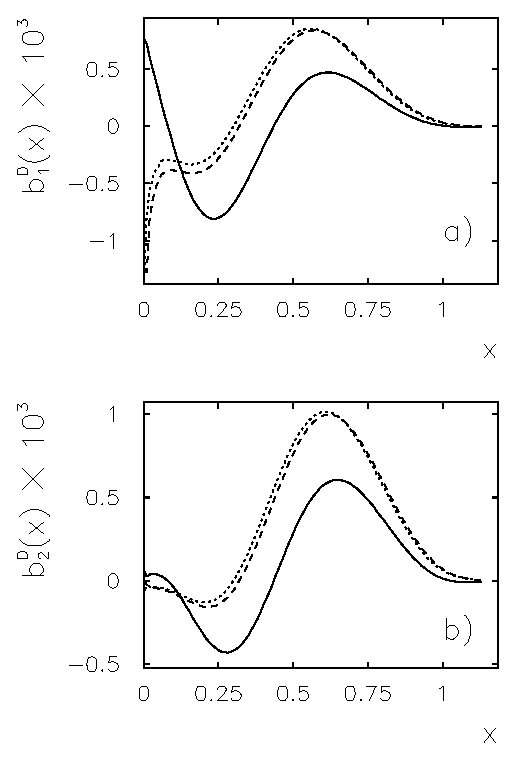
\includegraphics[width=0.3\textwidth]{figs/umnikov_b12.eps}
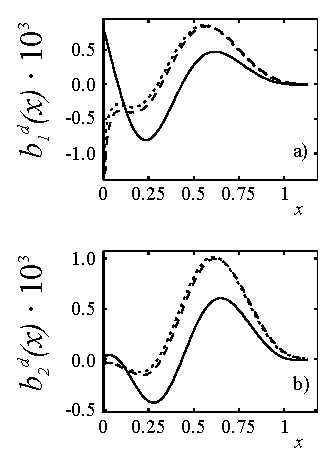
\includegraphics[width=0.35\textwidth]{newfigs/ellie/figure-6.eps}
\caption{\label{UMNIKOV} Relativistic convolution calculation of $b_1^D(x)$ and $b_2^D(x)$.  Curves: BS - solid, Bonn - dotted, Bonn with cut -dashed.
{\it Reproduced from Ref.~\cite{Umnikov:1996qv}.}
}
\end{center}
\end{figure}


%
\subsubsection{Double-Scattering Effects}
Using Vector Meson Dominance (VMD), the authors of Ref.~\cite{Bora:1997pi} isolate the 
double-scattering contribution to $b_1$. The existence time of a vector meson can 
be described by the coherence length: %$\lambda$: 
\begin{eqnarray}
\lambda = \frac{Q^2}{M x (M_v^2 + Q^2)}
\end{eqnarray}
which is the length over which the vector meson propagates during the time $\Delta t 
= 1/\Delta E$. For significant shadowing or double scattering to occur, a minimum coherence length 
of $\approx$ 1.7 fm (the inter-nucleon separation) is required. At 
$x > 0.3$, the coherence length is only about the size of the nucleon, so double
scattering contributions are anticipated to be negligible. However, for $x \le 0.1$, 
double-scattering should be significant in $b_1$ behaving as $(1-x)^{2\delta}/x^{1+2\delta}$, 
where $\delta$ is determined from the soft pomeron intercept $\alpha_P(t=0) = 1 + \delta$.
The authors predicted a significant enhancement of $b_1$ at low $x$ ($\le$ 0.01) 
due to the quadrupole deformation of the deuteron, which is qualitatively confirmed by the
HERMES data.  See Fig.~\ref{HERMES_AZZ}.
%\begin{figure}[t]
%\begin{center}
%\includegraphics[width=0.5\textwidth]{figs/bora_jaffe_fig3.eps}
%\caption{\label{b2_bora} Double-scattering contribution $b_2^{(2)}(x,Q^2)$ in 
%function of $x$~\cite{Bora:1997pi} (where $2 x b_1 = b_2 = b_2^{(1)}+b_2^{(2)}$).}
%\end{center}
%\end{figure}

\subsubsection{Virtual Nucleon Approximation}
  %Following the approach of Ref.~\cite{Frankfurt:1983qs},
M. Sargsian~\cite{MISAK} recently calculated the tensor asymmetry $A_{zz}$ for deep inelastic scattering.   
%Within the  PWIA approximation in which parton distributions in the deuteron  are generated
%due to partons in proton and neutron, he predicts no significant tensor asymmetry except at
%very large x (quasi-elastic scattering) in which case the D-wave becomes important. See Fig.~\ref{PROJ}.
%
See Fig.~\ref{PROJ}.  In the approximation in which  only proton-neutron component of the deuteron is taken into account and  nuclear parton distributions
are generated through the convolution of partonic distribution of nucleon and deuteron density matrix (see e.g. Refs.~\cite{Frankfurt:1981mk,Sargsian:2001gu}), %       FS81,SSS},   
the deuteron structure function $b_1$ is related directly to the d-partial wave of the deuteron wave function~\cite{MISAK,Frankfurt:1981mk}.   %\cite{FS81,MS}.  
As a result,  this approximation predicts negligible  magnitude for $b_1$  for $x\le 0.6 $ due to small Fermi momenta involved  in the convolution integral. 
However, the predicted magnitude of $b_1$ is large at $x \ge 0.7$ where one expects substantial contribution from the d-waves due to 
high momentum component of the deuteron wave function involved in the convolution picture of DIS scattering off the deuteron.
In this case, $b_1$ is very sensitive to the relativistic description of the deuteron and its measurement can be used for checking 
the different approximations of high momentum  component of deuteron wave function.  

In the calculation presented, two Virtual Nucleon  and Light-Cone approximations are used to calculate the  tensor polarization for 
DIS scattering off the deuteron.  In both approximations only the proton-neutron component of the deuteron is taken into account.
In the Virtual Nucleon approximation, the covariant scattering amplitude is reduced  by estimating the spectator nucleon 
propagator at its on-energy shell in the lab frame of the deuteron.  Within this approximation the baryonic sum rule is satisfied while the 
momentum sum rule is not. The latter is due to the fact that part of the light cone momentum of the bound  virtual nucleon is lost to the 
unaccounted non-nucleonic degrees of freedom in the deuteron wave function.
In the light cone approximation the scattering amplitude is estimated the $E+p_z$ pole of the spectator nucleon on the light cone.
In this case the wave function is defined on the light-cone reference frame and it satisfies both baryon number and momentum sum rules.
For the detailed comparison  of these approximations, see Ref.~\cite{Sargsian:2001gu}.   %~\cite{SSS}.



\subsubsection{Fit to HERMES  Data}
Kumano~\cite{Kumano:2010vz} points out that the twist-2 structure functions $b_1$ and $b_2$ can be used to probe orbital angular momentum.  
He then extracts the tensor polarized quark and anti-quark distributions from a fit to the HERMES data~\cite{Airapetian:2005cb}. 
He finds that a non-negligible tensor polarization of the sea is necessary to reproduce the trend of
the data, as shown in Fig.~\ref{xb1_pred}. However, this conclusion has to be considered with caution due to the extended
$Q^2$ coverage (Fig.~\ref{HERMES_KIN}), and large uncertainty of each HERMES data point.
In particular, the author calls for better measurements of $b_1$ at large $x$ ($>0.2$), and further investigation of
the tensor structure functions in general.

\subsubsection{The Close-Kumano Sum Rule}
\label{CKSEC}
Following the formalism from the parton model in~\cite{Hoodbhoy:1988am}, Close and
Kumano~\cite{Close:1990zw} related the tensor structure function $b_1$ to the electric quadrupole
form factor of the spin-1 target through a sum rule\footnote{Efremov and Teryaev evidently proposed the same relation for
mesons in Ref.~\cite{Efremov:1981vs}.}:
\begin{eqnarray}
\int_0^1 dx~b_1(x)  & = &  - \frac{5}{12 M^2} \lim_{t \rightarrow 0}~t~F_Q(t)
                           + \frac{1}{9} \Big(\delta Q + \delta \bar{Q}\Big)_s \nonumber \\
                    & = & \frac{1}{9} \Big(\delta Q + \delta \bar{Q}\Big)_s  = 0 
\label{cksum}
\end{eqnarray}
where $F_Q(t)$ is the electric quadrupole form factor of a spin-1 hadron at the momentum squared $t$. 
The Close Kumano (CK) sum rule is satisfied in the case of an unpolarized sea. The authors note
that in nucleon-only models, the integral of $b_1$ is not sensitive to the
tensor-polarization of the sea, and consequently the sum rule is always true, even when the
deuteron is in a $D$-state.

The authors of Ref.~\cite{Khan:1991qk} calculated 
the first moment of $b_1(x)$ in a
version of the convolution model that incorporates relativistic and binding energy corrections.  They found a value of -6.65$\cdot 10^{-4}$, and
emphasize that deviations from this will serve as a good signature of exotic effects in the deuteron wave function.  Similarly, Ref.~\cite{Umnikov:1996qv} predicts $5\cdot 10^{-4}$ and  $3\cdot 10^{-5}$ for the relativistic and nonrelativistic calculation of Eq.~\ref{cksum}, respectively.




A truncated version of Eq.~\ref{cksum} was evaluated by the HERMES~\cite{Riedl:2005jq,Airapetian:2005cb} experiment and found to be:
\begin{eqnarray}
\int_{0.0002}^{0.85} b_1(x) dx = 0.0105 \pm 0.0034 \pm 0.0035
\end{eqnarray}
which possibly indicates a breaking of the Close-Kumano sum rule, and consequently a
tensor-polarized quark sea.  However, since the comparison is only at the two sigma level,  more precise data is needed for a true test.


%

\subsubsection{Angular Momentum Sum Rule for Spin-1 Hadronic Systems}

The $b1$ structure function is connected with the spin-1 angular momentum sum rule as discussed in Ref.~\cite{Taneja:2011sy}.
By examining the energy momentum tensor for the deuteron, the authors showed that 
it was possible to define an additional sum rule for $b_1$ (see Eq. 12 in Ref.~\cite{Taneja:2011sy}) where it was shown that the second moment of this quantity is non vanishing, being related to one of the gravitomagnetic deuteron form factors.  A measurement of $b_1$ would provide a unique test of this idea.

It is also important to notice that $b_1$ singles out the role of the $D$-wave component in distinguishing coherent nuclear effects through tensor polarized correlations  from  the independent nucleon's partonic spin structure.
A similar role of the D-wave component was also found in the recently proposed spin sum rule where it plays a non-trivial role
producing a most striking effect through the spin flip GPD E. An experimental measurement of $b_1$ would corroborate this scenario.



\newpage
\subsection{Interest from Theorists}
%
During the preparation of this proposal, we contacted several theorists 
to gauge interest in a precision measurement of $b_1$.  The response was uniformly positive.  We 
provide some of their feedback for context.
%
%\vspace{0.5cm}
%{\bf S. Kumano (KEK and Tsukuba U.):}
%\vspace{0.5cm}
%{\bf M. Strikman (Penn. State U.) and M. Sargsian (FIU):}
%

\vspace{0.5cm}
\noindent
{\it 
%The tensor structure of the deuteron can be investigated in the deep
%inelastic region by measuring the structure function $b_1$, which
%should shed light on a new aspect of tensor-structure studies in
%terms of quark degrees of freedom instead of hadronic ones.
%There is a conventional approach for theoretically calculating $b_1$
%by quark distribution functions convoluted with nucleon momentum
%distributions in the deuteron including the $D$-state admixture.
%According to our experience on the nucleon-spin issue, such
%a conventional approach for high-energy spin physics would not work.
%In particular, 
It is known that $b_1$ is sensitive to dynamical aspects
of constituents with angular momenta. 
%
Measurements of $b_1$ could open
a new field of spin physics because this kind of spin physics has not
been explored anywhere else. The only experimental information came from
the HERMES collaboration; however, their data are not accurate enough
to find the $x$ dependence of $b_1$, especially at large $x$. 

It is an unique opportunity at JLab to develop this new field of spin physics.

%I think that your experiment should be an important one
%for opening a few field of hadron physics.
%so I hope that your proposal will be accepted.
}
\begin{flushright}{\bf S. Kumano (KEK)}\end{flushright}

\vspace{0.5cm}
\noindent
{\it I'm glad to hear that $b_1$ is not forgotten in all the excitement about other spin dependent 
effects.
%I don't have much to add to the existing discussion of $b_1$ in the literature. 
%If I remember correctly, 
%The hard thing is to distinguish a non-trivial contribution to $b_1$ (eg. 
%from 6 quark correlations in the deuteron) from the contribution from the deuteron d-wave.
}
%I 
%also remember a debate about a double scattering contribution.  I wrote a paper on that subject 
%with an Indian visitor to the CTP.  I believe our work was a follow-on to work by Nikolaev and 
%Schafer~\cite{Nikolaev:1996jy}.  I think these papers suggested large contributions to $b_1$ at 
%low x and low $Q^2$.}''
\begin{flushright}{\bf R. Jaffe (MIT)}\end{flushright}

\vspace{0.5cm}
\noindent{\it I am particularly interested in signatures of novel QCD effects in the deuteron. The tensor 
charge could be sensitive to hidden color (non-nucleonic) degrees of freedom at large $x$. It is
also interesting that antishadowing in DIS in nuclei is not universal but depends on the quark 
flavor and spin. One can use counting rules from PQCD to predict the $x \to 1$ dependence of the 
tensor structure function.}
\begin{flushright}{\bf S. Brodsky (SLAC)}\end{flushright}
 
\vspace{0.5cm}
\noindent{\it I am certainly interested in the experimental development to find the novel
QCD phenomena from the hidden color component of deuteron.}
\begin{flushright}{\bf Chueng-Ryong Ji (NCSU)}\end{flushright}

\vspace{0.5cm}
\noindent{\it You have finally piqued my interest in this subject...Surely this 
is of real interest the spin community!  I hope I might be able to say something coherent
about the partonic interpretation at some point--this of course is where my real interest lays.}
\begin{flushright}{\bf Leonard Gamberg (Penn State Berks)}\end{flushright}

\vspace{0.5cm}
\noindent{\it I find the proposal well written, well justified, sound, and exciting.}
\begin{flushright}{\bf Alessandro Bacchetta (Universita di Pavia)} \end{flushright}




\section{The Proposed Experiment}

\subsection{Experimental Method} %Measurement of $A_{zz}$ }

The measured double differential cross section for a spin-1 target is characterized by a vector polarization $P_{z}$ and tensor polarization
$P_{zz}$ is expressed as,
\begin{equation}
\frac{d^2\sigma_p}{d\Omega dE'}=\frac{d^2\sigma_u}{d\Omega dE'}\left(1-P_zP_BA_1+\frac{1}{2}P_{zz}A_{zz}\right),
\label{eq:one}
\end{equation}
where, $\sigma_p$ ($\sigma_u$) is the polarized (unpolarized) cross section, $P_B$ is the incident electron beam polarization, and $A_1$ ($A_{zz}$) is the
vector (tensor) asymmetry of the virtual-photon deuteron cross section.  This allows us to write
the polarized tensor asymmetry with $0<P_{zz}\leq 1$ using an unpolarized electron beam as
\begin{eqnarray}
\label{Azz}
A_{zz} = \frac{2}{P_{zz}}\left(\frac{\sigma_p - \sigma_u}{\sigma_u}\right).
\end{eqnarray}
The tensor polarization is given by 
\begin{equation}
P_{zz}=\frac{n_+-2n_0+n_-}{n_++n_-+n_0},
\end{equation}
where $n_m$ represents the population in the $m_z=+1$,~$-1$,~or $0$ state.

Eq. \ref{Azz} reveals that the asymmetry $A_{zz}$ compares two different cross sections measured under different polarization conditions of the target: positively tensor polarized and unpolarized.  
To obtain the relative cross section measurement in the same configuration, the same target cup and material will be used at alternating polarization states (polarized vs. unpolarized),  and the magnetic field providing the quantization axis will be oriented along the beamline at all times.
This field will always be held at the same value, regardless of the target material polarization state. 
This process, identical to that used for the E12-13-011 $b_1$ measurement, ensures that the acceptance remains consistent within the stability (10$^{-4}$) of the super conducting magnet.  


Since many of the factors involved in the cross sections cancel in
the ratio, Eq. \ref{Azz} can be expressed in terms 
of the charge normalized, efficiency corrected numbers of tensor polarized ($N_p$) and unpolarized ($N_u$) counts, 
\begin{eqnarray} \label{3}
A_{zz}&=&\frac{2}{fP_{zz}}\left(\frac{N_p - N_u}{N_u}\right) .
\end{eqnarray}

The dilution factor $f$ corrects for the presence of unpolarized nuclei in the target and is defined by
\begin{equation}
f=\frac{N_D\sigma_D}{N_N\sigma_N+N_D\sigma_D+\sum\limits_{A} N_A\sigma_A},
\end{equation}
where $N_D$ is the number of deuterium nuclei in the target and $\sigma_D$ is the corresponding inclusive double differential scattering cross 
section, $N_N$ is the nitrogen number of scattered nuclei with cross section $\sigma_N$, and $N_A$ is the number of other scattering nuclei of mass number $A$ with cross section $\sigma_A$. As has been noted in previous work~\cite{Frankfurt:1988nt}, the dilution factor at high $x$ drops off considerably until the SRC plateau region, as shown in Fig.~\ref{fdil}. By using a high-luminosity solid target and a low scattering angle $\theta_{e'}$, this effect will be counteracted.

\begin{figure}
\begin{center}
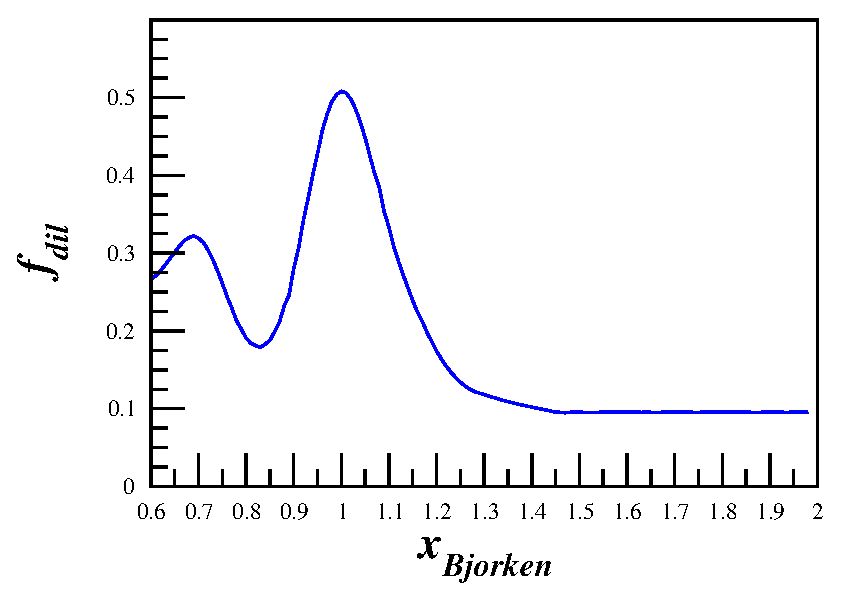
\includegraphics[width=0.45\textwidth]{figs/fdil_q2_15.eps}
\caption{\label{fdil}The estimated dilution factor, in this case at $Q^2=1.5 \mathrm{~(GeV}/c)^2$, is expected to drop off at high $x$ until it reaches the SRC plateau region. This effect will be counteracted by using a high-luminosity solid target.}
\end{center}
\end{figure}

The dilution factor can be written in terms of the relative volume ratio of ND$_3$ to LHe in the target cell, otherwise known as the packing fraction $p_f$.  
In our case of a cylindrical target cell oriented along the magnetic field,the packing fraction is exactly equivalent to the percentage of the cell length filled with ND$_3$.  
%The dilution factor is discussed in further detail in Sec. \ref{dil}.

If the time is evenly split between scattering off of polarized and unpolarized ND$_3$, the time necessary to achieve the desired precision $\delta A$ is:
\begin{equation}
T=\frac{N_p}{R_p}+\frac{N_u}{R_u}=\frac{8}{f^2P_{zz}^2}\left(\frac{R_p(R_u+R_p)}{R_u^3}\right)\frac{1}{\delta A_{zz}^2}
\end{equation} 
where $R_{p(u)}$ is the polarized (unpolarized) rate and $N_{p(u)}$ is the total estimated 
number of polarized (unpolarized) counts to achieve the uncertainty $\delta A_{zz}$.  

%See Sec.~\ref{stat} for full details of the statistical uncertainty.



%\begin{table}
%\begin{center}
%\begin{tabular}{c|ccc|cc|c|cc|cc|c}
%& $\overline{x}$  & $\overline{Q^2}$      &  $\overline{W}$  &    $P_0$    &    $\theta$  &  Rates & $A_{zz}$ & $\delta A_{zz}^{stat}$    & $b_1$  & $\delta b_1^{stat}$ & time   \\
%&  ~     & (GeV$^2$)  & (GeV) & (GeV)  &     (deg.)  &   (kHz)  & \multicolumn{2}{|c|}{$\times 10^{-2}$} &  \multicolumn{2}{|c|}{$\times 10^{-2}$}    & (days) \\
%%\multicolumn{2}{|c|}{$\times 10^{-2}$}
%\hline\hline
%SHMS & 0.30&  1.5&  2.11&  8.46&     7.3&    0.48&   0.48&   0.11&  -0.33&   0.072&   15.7 \\
%SHMS & 0.40&  2.2&  2.07&  8.20&     9.0&    0.14&   0.99&   0.22&  -0.38&   0.083&   12.5 \\
%HMS  & 0.50&  3.5&  2.11&  7.30&    12.2&    0.03&   1.40 &   0.34&  -0.25&   0.062&   28.1 \\
%
%\hline\hline
%\end{tabular}
%\caption{\label{RATES}OLD TABLE. NEEDS TO BE UPDATED. Summary of the kinematics and physics rates using Hall C  spectrometers.}
%\end{center}
%\end{table}


\begin{table}
\begin{center}
\begin{tabular}{c|c|c|c|cc|c|c}
& $\overline{x}$  & $\overline{Q^2}$    &  $\overline{W}$  	& $P_0$  &    $\theta$  &  Rates   & PAC Time   \\
&  ~     		  & (GeV$^2$)  			& (GeV) 			& (GeV)  &     (deg.)   &   (kHz)  & (days) \\
%\multicolumn{2}{|c|}{$\times 10^{-2}$}
\hline\hline
%Spec    x     Q2		W		P0		 Theta		 Rates		Time
HMS  & 0.90	&  1.3	&  1.01	&  5.83	&    10.55	&    0.88	&   14 \\  
SHMS & 1.30	&  1.3	&  0.76	&  6.07	&    10.34	&    0.43	&   14 \\
\hline\hline
\end{tabular}
\caption{\label{RATES1}Summary of the kinematics and physics rates using the Hall C  spectrometers.}
\end{center}
\end{table}


\begin{table}
\begin{center}
\begin{tabular}{c|c|c|c|c}
 $\overline{x}$  & $\overline{Q^2}$  &  $\overline{W}$ & $f_{dil}$ & $\delta A_{zz}^{stat}$ \\
     & (GeV$^2$)  & (GeV) &  & $\times 10^{-2}$  \\
\hline\hline
%    x  		   Q2		W	   fdil 	   dAzz 
    0.80		&  1.30	&  1.09 &  0.177	 & 0.62	\\
    0.90		&  1.30	&  1.01 &  0.293	 & 0.37	\\
    1.00		&  1.30	&  0.94 &  0.512	 & 0.20	\\
    1.10		&  1.30	&  0.88 &  0.346	 & 0.41	\\  
    1.20		&  1.30	&  0.83 &  0.180	 & 1.10	\\  
    1.30		&  1.30	&  0.78 &  0.108	 & 2.38	\\  
    1.40		&  1.30	&  0.73 &  0.071	 & 4.74	\\  
    1.55		&  1.30	&  0.67 &  0.046	 & 7.02	\\              
    1.75		&  1.30	&  0.59 &  0.034	 & 13.8	\\  
\hline\hline
\end{tabular}
\caption{\label{RATES2}Summary of the expected statistical uncertainty after combining overlapping x-bins.  Values represent the statistics weighted average of all events that satisfy our kinematic cuts. }
\end{center}
\end{table}




\label{EXP}
We will measure the tensor asymmetry \Azz for $\XMIN<x<\XMAX$, $\QMIN$~(GeV/$c)^2 < Q^2 <\QMAX$~(GeV/$c)^2$ and $\WMIN < W < \WMAX$~GeV. Fig.~\ref{kincov} shows the planned kinematic coverage utilizing the Hall C HMS and SHMS spectrometers at forward angle.

\begin{figure}
\begin{center}
%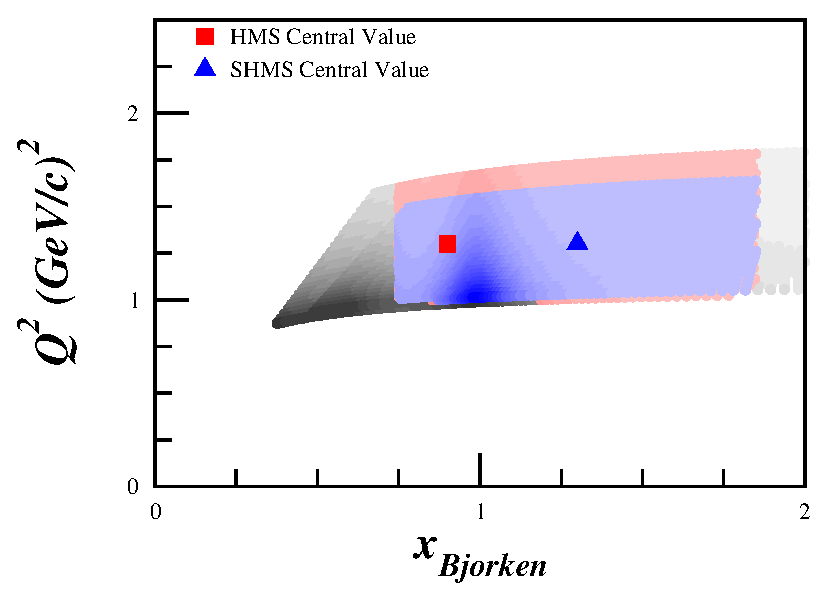
\includegraphics[width=0.49\textwidth]{figs/kine/Pzz_30_q2.eps}~~ %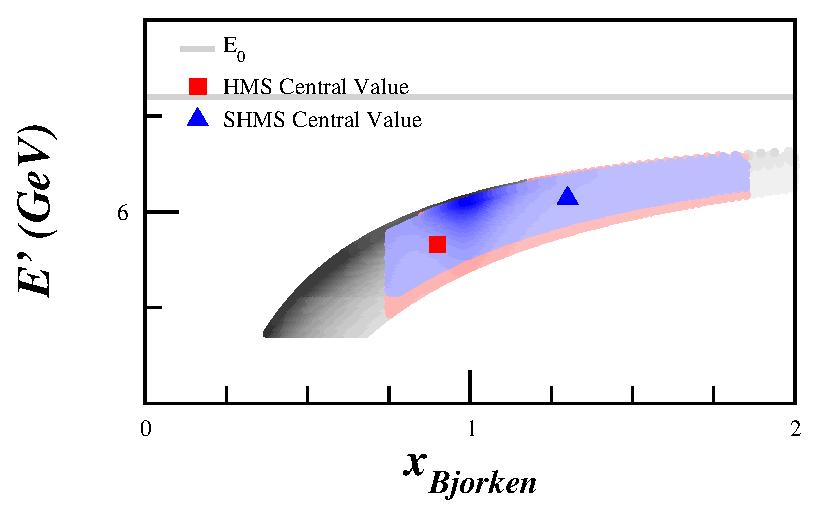
\includegraphics[width=0.49\textwidth]{figs/kine/Pzz_30_eprime.eps}
%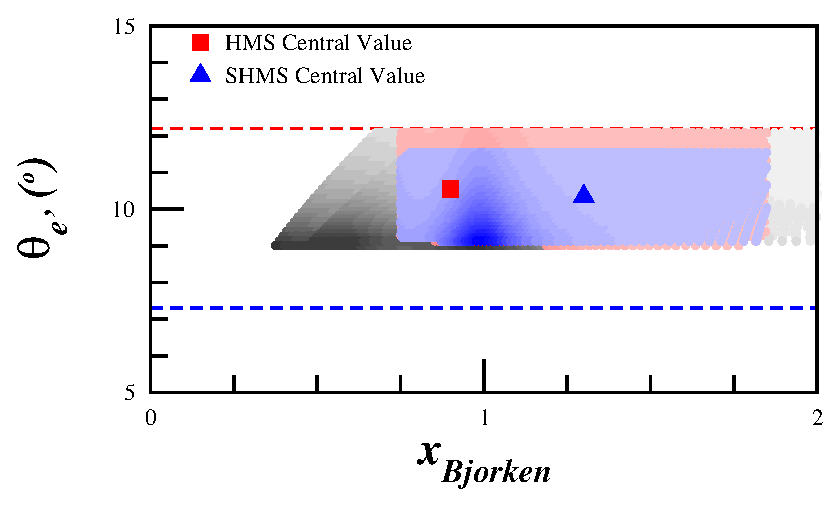
\includegraphics[width=0.49\textwidth]{figs/kine/Pzz_30_theta_eprime.eps}~~ 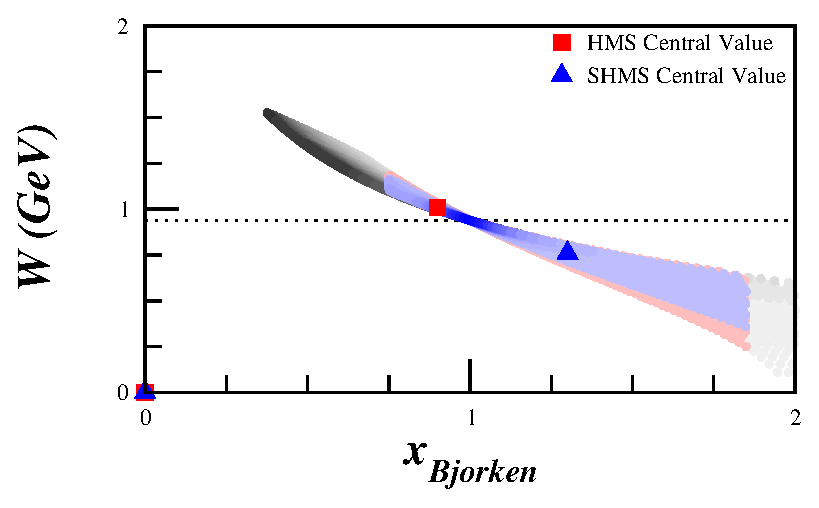
\includegraphics[width=0.49\textwidth]{figs/kine/Pzz_30_w.eps}
\caption{\label{kincov} Kinematic coverage.  The grey settings are not included in our rates estimates since they fall outside of $\XMIN < x < \XMAX$. The highlighted represent the central value of the spectrometer setting, which are not the statistics weighted average of the distribution. The shading represents areas with greater statistics.}
\end{center}
\end{figure}


The polarized \TARGET target is discussed in section~\ref{POLTARGSEC}.  The magnetic field of the target will be held constant along the beamline at all times, while the target state is alternated between a polarized and unpolarized state.
The tensor polarization and packing fraction used in the rates estimate are \PZZ\% and \PF, respectively. 
The packing fraction changes with $x$ in the range of this measurement as shown in Fig.~\ref{fdil_plot}.
With an incident
electron beam current of \CURRENT nA, the
expected deuteron luminosity is $1.57\times 10^{35}$ / cm$^2\cdot$s$^1$. The momentum bite and the acceptance
were assumed to be $\Delta P = \pm 8\%$ and $\Delta\Omega = 5.6$ msr for the HMS, and $\Delta P= ^{+20\%}_{-8\%}$ 
%$-8<\Delta P <+20\%$
and $\Delta\Omega =4.4$ msr for the SHMS. 
%
For the choice of the kinematics,
special attention was taken onto the angular and momentum limits of the spectrometers: for the
HMS, $10.5^{\circ} \le \theta \le 85^{\circ}$ and $1 \le P_0 \le 7.3$ GeV/c, and for the SHMS,
$5.5^{\circ} \le \theta \le 40^{\circ}$ and $2 \le P_0 \le 11$ GeV/c. In addition, the
opening angle between the spectrometers is physically constrained to be larger than 17.5$^{\circ}$.
The invariant mass $W$ was kept to $W \ge \WMIN$ GeV for all settings.
The projected 
uncertainties and $A_{zz}$
are summarized in Table~\ref{RATES2}, and displayed in
Fig.~\ref{PROJ}.  

\begin{figure}
\begin{center}
%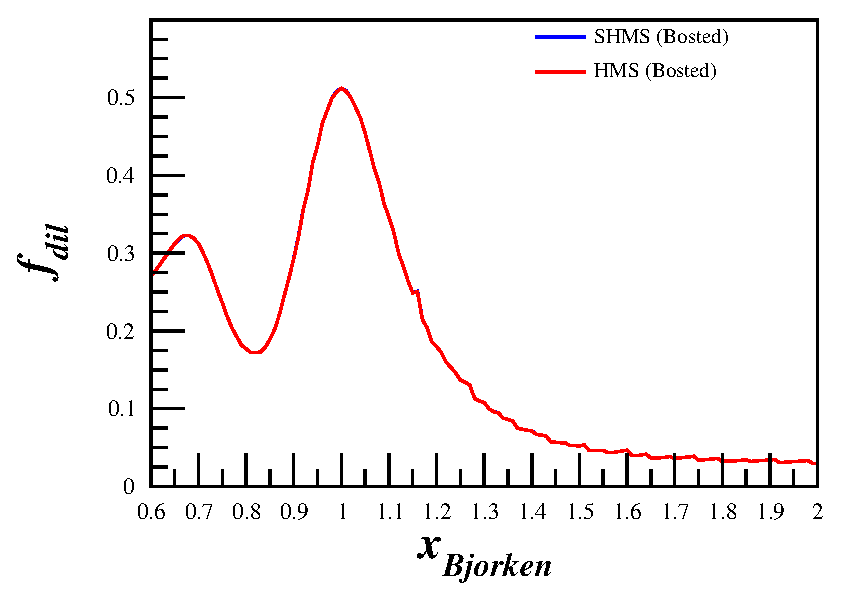
\includegraphics[width=0.5\textwidth]{figs/kine/Pzz_30_fdil.eps} 
\caption{\label{fdil_plot}Projected dilution fraction covering the entire $x$ range to be measured using the Bosted fits \cite{Bosted:2012qc} for the SHMS and HMS. In the kinematics used, both dilution factors overlap.}
\end{center}
\end{figure}

\begin{figure}
\begin{center}
%\includegraphics[width=0.45\textwidth]{figs/plots0705/b1_proj_newmiller_lin.eps}
%\hspace{0.5cm}
%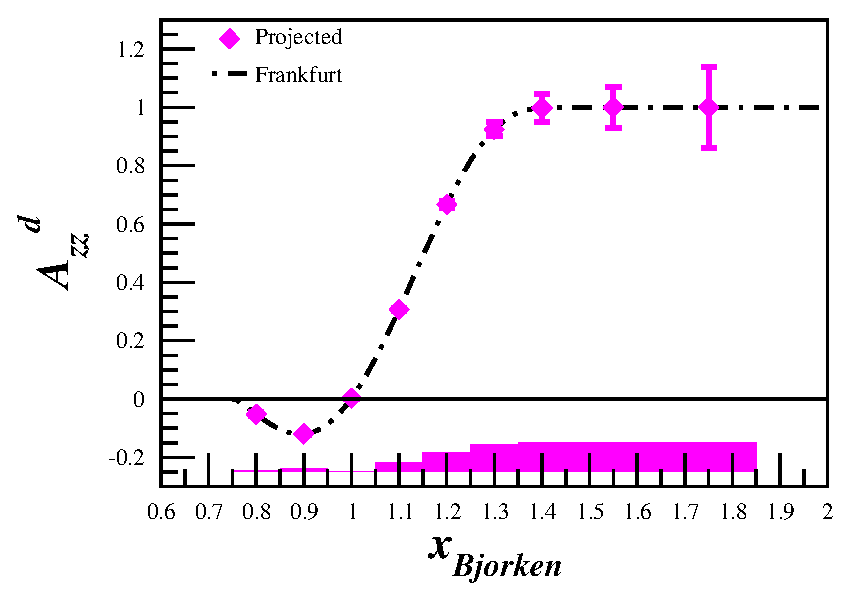
\includegraphics[width=0.5\textwidth]{figs/kine/Pzz_30_Azz_nobars.eps} 
\caption{\label{PROJ}Projected statistical errors for the tensor asymmetry $A_{zz}$ with \productiondays days of beam time. Data at different $Q^2$ are combined with an x-binning that varies slightly per point, but is approximately $\pm0.05$. The band represents the systematic uncertainty. Also shown are the calculations from Frankfurt and Strikman \cite{Frankfurt:1988nt}.
}
\end{center}
\end{figure}

A total of 
\productiondays
 days of beam time is requested for production data, with an additional \overheaddays days of expected overhead.



\clearpage

%







\subsection{Uncertainty Estimates}
\subsubsection{Statistical Uncertainty}
\label{stat}
To investigate the statistical uncertainty we start with the equation for $A_{zz}$ using
measured counts for polarized data ($N_p$) and unpolarized data ($N_u$), 
\begin{equation}
A_{zz}=\frac{2}{fP_{zz}}\left(\frac{N_p}{N_u}-1\right).
\end{equation}
The statistical error with respect to counts is then
\begin{equation}
\delta A_{zz}=\frac{2}{fP_{zz}}\sqrt{\left(\frac{\delta N_p}{N_u}\right)^2+\left(\frac{N_p\delta N_u}{N_u^2}\right)^2}.
\end{equation}
For $\delta N_{p(u)}=\sqrt{N_{p(u)}}$, the uncertainty becomes
\begin{equation}
\delta A_{zz}=\frac{2}{fP_{zz}}\sqrt{\frac{N_p(N_u + N_p)}{N_u^3}},
\end{equation}
which can't be simplified further due to the large expected asymmetry.


\subsubsection{Systematic Uncertainty}% in $A_{zz}$ }
\begin{table}
\begin{center}
\begin{tabular}{l|c}\hline\hline
Source								& Systematic \\
\hline
$P_{zz}$ Polarimetry					& 12\%   \\
Dilution Factor						& 6.0\%   \\
Packing Fraction						& 3.0\%   \\
Trigger/Tracking Efficiency			& 1.0\% \\
Acceptance							& 0.5\% \\
Charge Determination					& 1.0\%  \\
Detector Resolution and Efficiency	& 1.0\% \\
\hline
Total								& 14\%   \\
\hline
\end{tabular}
\caption{\label{error1}Estimates of the scale dependent contributions to the systematic error of $A_{zz}$.}
\end{center}
\end{table}

Table \ref{error1} shows a list of the scale dependent uncertainties contributing to the systematic error in $A_{zz}$.
With careful uncertainty minimization in polarization the relative error in vector polarization, $Pz$, can be less than or equal to 3.9\%, as demonstrated in the recent E08-027/E08-007 experiment~\cite{NIMDUST} and nearly as good for the deuteron using multiple techniques to measure the NMR signal as discussed in ~\cite{PTSTDUST}.  With the use of a positive tensor enhanced target it has been projected to be able to achieve a relative error in $P_{zz}$ better than 12\% ~\cite{PTSTDUST}.  The uncertainty from the dilution in the polarized target is estimated to be
about 6\% over the range of kinematics points of interest.  We consider separately the uncertainty in the packing fraction of the ammonia target contributes at a level of less than 3\%. Charge calibration and detector efficiencies are expected to be known better to 1\%. 
%but the impact of time-dependent drifts in these quantities must be carefully controlled.

\subsubsection*{Time Dependent Systematic Effects}
Eq.~\ref{3} involves the ratio of counts, which leads to cancellation of several first order systematic effects.  However, the fact that the two data sets will not be taken simultaneously leads to a sensitivity to time dependent variations which will be monitored and suppressed. While typical false asymmetries in Hall C of $0.01$ are acceptable for this proposed measurement, we are interested in a strict control of the systematics for further reduction.
%
To investigate the systematic differences in the time dependent components of the integrated counts, we need to consider the effects from calibration, efficiency, acceptance, and luminosity between the two polarization states.

Fluctuations in luminosity due to target density variation can easily be kept to a minimum by keeping the material beads at the same temperature for both polarization states by control of the microwave and the LHe evaporation.  The He vapor pressure reading gives accuracy of material temperature changes at the level of $\pm0.1\%$.
%Beam rastering can also be controlled to a high degree.

The beam charge asymmetries between two helicity states using the luminosity monitors for experiment
E06-010 has been shown to be at the level of $4 \times 10^{-5}$ with a width of $2 \times 10^{-4}$.
An additional estimate on the change in the BCM calibration constant is seen in
experiment E08-027 resulting in a absolute deviation of $2 \times 10^{-4}$ over the course of six
days. We expect to be able to minimize long term drifts by careful thermal isolation of
the BCMs.
%, however resulting trends will be studied and corrections implemented.

The acceptance of each cup can only change as a function of time if the magnetic field changes.  
The capacity to set, reset, and hold the target superconducting magnet to a desired holding field causes a field uncertainty of $\delta B /B=0.01\%$. 
This implies that, like the cup length $l$, the acceptance ${\cal A}$ for each polarization state is the same.

In order to look at the effect on $A_{zz}$ due to drifts in beam current monitor calibration and detector efficiency, we rewrite Eq.~\ref{3} explicitly in terms of the raw measured counts $N_p^c$ and $N_u^c$,
\begin{eqnarray} \label{3c}
\nonumber
A_{zz}&=&\frac{2}{fP_{zz}}\left(\frac{N^c_p}{N^c_u}-1\right) \\
      &=&\frac{2}{fP_{zz}}\left(\frac{Q\varepsilon l \cal{A}}{Q_1\varepsilon_1 l \cal{A}}\frac{N_p}{N_u}-1\right)
\end{eqnarray}
where $Q$ represents the accumulated charge, and $\varepsilon$ is the detector efficiency. The target length $l$ and acceptance $\cal{A}$ are identical in both states to first order.

We can then express $Q_1$ as the change in beam current measurement calibration that occurs in
the time it takes to collect data in one polarization state before switching to another, such that $Q_1=Q(1-dQ)$.
In this notation, $dQ$ is a dimensionless ratio of changes in different polarization states and would ideally be equal to zero.  A similar representation
is used for drifts in detector efficiency leading to,
\begin{equation}
A_{zz}=\frac{2}{fP_{zz}}\left(\frac{N_pQ(1-dQ)\varepsilon(1-d\varepsilon)}{N_u Q\varepsilon}-1\right).
\end{equation}
which simplifies to,
\begin{equation}
A_{zz}=\frac{2}{fP_{zz}}\left(\frac{N_p}{N_u}(1-dQ-d\varepsilon+dQd\varepsilon)-1\right).
\end{equation}

We obtain estimates of $dQ$ and $d\varepsilon$ from previous experimental
studies.  During the JLab transversity experiment E06-010, the detector drift was measured such that the normalized yield over a three month period indicated little change ($<1$\%).
These measurement were then used to show that for short time (20 minutes periods between target spin flip),
the detector drift was estimated to be less than 1\% times the ratio of the time period between target spin flip and three months.
For the present experiment we use the same estimate except for the period between target polarization states used is
$\approx 36$ hours leading to an overall drift $d\varepsilon\approx 0.01\%$.  A similar approach is used to establish an estimate
for $dQ$ using studies from the data from the E08-027 experiment resulting in $d\varepsilon \approx 0.01\%$.

To express $A_{zz}$ in terms of the estimated experimental drifts in efficiency and current measurement we can write,
\begin{equation}
A_{zz}=\frac{2}{fP_{zz}}\left(\frac{N_1}{N}-1\right)\pm\frac{2}{fP_{zz}}d\xi.
\end{equation}
This leads to a contribution to $A_{zz}$ on the order of $1\times10^{-3}$,
\begin{equation}
dA_{zz}^{drift}=\pm\frac{2}{fP_{zz}}d\xi=\pm3.7\times10^{-3}.
\end{equation}
%For this estimate we assume only two polarization state changes in a day. If it is possible to increase this rate then the systematic effect in $A_{zz}$ will decrease accordingly.

Naturally detector efficiency can drift for a variety of reasons, for
example including fluctuations in gas quality, HV drift or
drifts in the spectrometers magnetic field.  All of these types of variation as can be realized both
during the experiment though monitoring as well as systematic studies of the data collected.
Checks on the consistency of the cross section data that can be use ensuring the quality of each run will be used in the asymmetry analysis.  Regression can be use to correct for any long term drifts that are of a non-stochastic nature.
Each of these systematic effects can mitigate the systematic uncertainty to $\sim0.001$. 
In the kinematic region proposed here, $A_{zz}$ is expected to be large, on the order of $0.1$ to $1.0$, making any absolute errors on this scale only critical as the data and models pass through the x-axis.  

\subsection{Polarized Target}
\label{POLTARGSEC}
This experiment will use the
JLab/UVa dynamically polarized solid {\TARGET}target operated in longitudinal mode.  
%Transverse polarization requires  operation of an upstream chicane to ensure proper transport through the target magnetic field.  
The target is typically operated with a specialized slow raster and beamline instrumentation capable of characterizing the low current 50-100 nA beam.
All of these requirements have been met previously in Hall C.
%, and will be soon implemented also in Hall A for the E08-027/E08-007 run in 2011. 
%
The polarized target (see Fig.~\ref{fig:target}), 
has been successfully used in experiments E143, E155, and E155x at SLAC, and E93-026, E01-006 and E07-003, E08-027 and E08-007 at JLab.
A similar target was used in Hall B for the EG1, EG4, and DVCS experiments. 
%although Hall B does
%not at present have the facilities necessary to operate a transversely polarized target with an electron beam.

The JLab/UVa target underwent significant renovation and improvement~\cite{CKEITH} during the recent g2p run. The magnet was replaced early in the run, and the target then performed consistently at or above historical levels.   A new 1 K refrigerator and target insert were designed and constructed by the JLab target group.  The cryogenic pumping system has been overhauled.  In particular, the older Alcatel 2060H rotary vane pumps have been replaced with new Pfeiffer DU065 magnetically coupled rotary vane pumps, and the pump controls are being refurbished. The target motion system has been rebuilt from scratch. %And now, the magnet and vacuum jacket rotate independently of the refrigerator and target insert, which simplifies rotation from parallel to perpendicular magnetic field orientations.

%
\begin{figure}
\centering
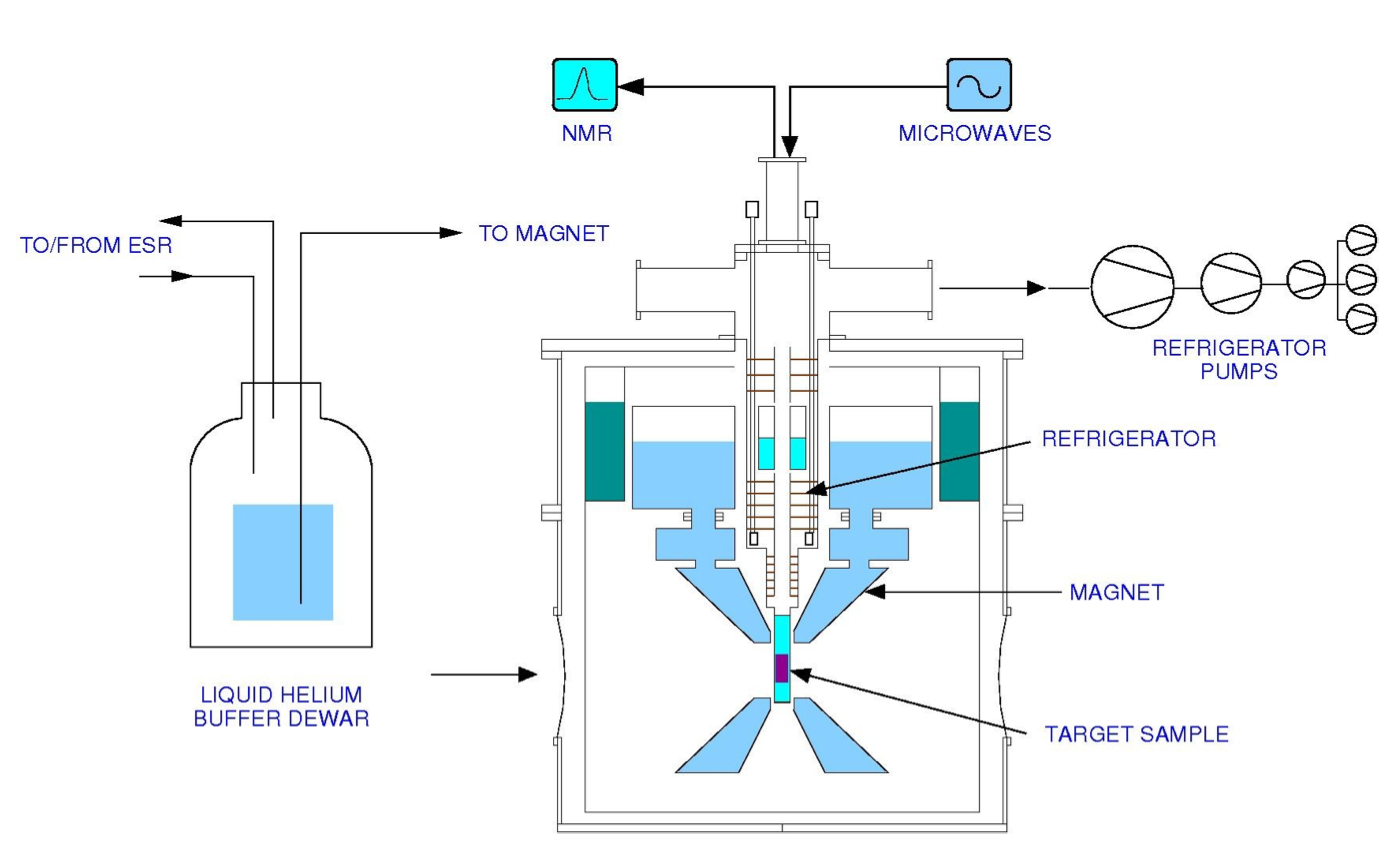
\includegraphics[width=5.0in,clip]{figs/targnew.eps} %target_gimp.eps}
\caption{Cross section view of the JLab/UVa polarized target. Figure courtesy of C. Keith.  \label{fig:target}}
\end{figure}


%\begin{figure}
%\centering
%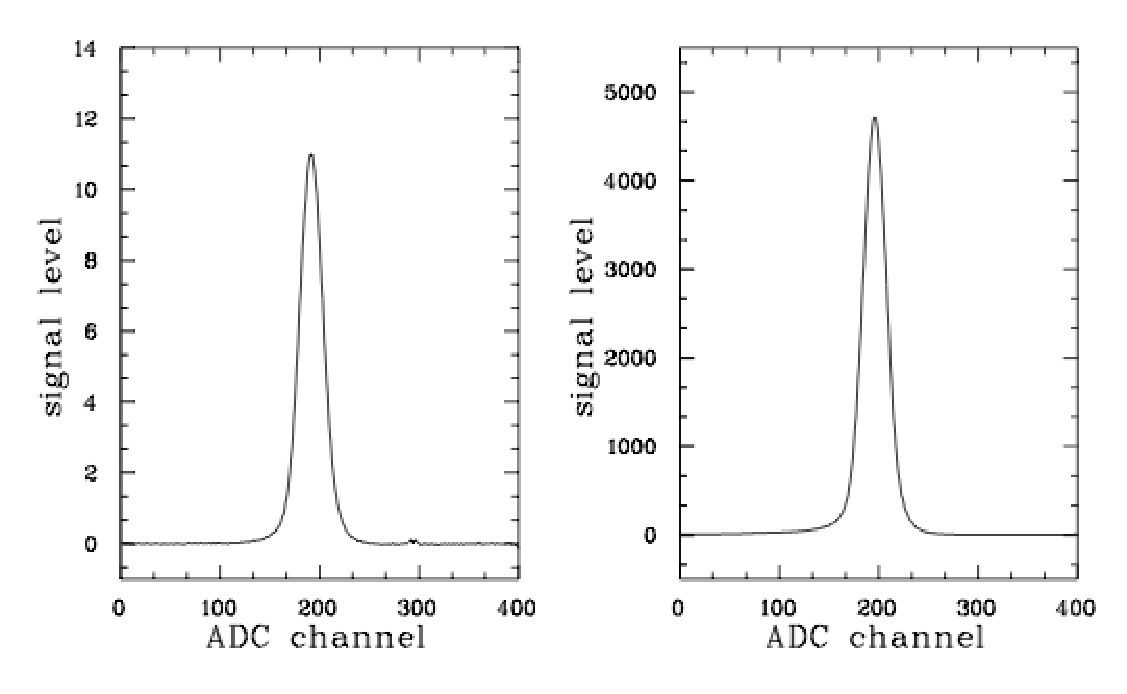
\includegraphics[width=4.5in,clip]{figs/liD.eps}
%\caption{\label{fig:LID} Typical Deuteron thermal equilibrium (TE) and enhanced signals in $^6$LiD.  The left plot shows a typical deuteron TE and the right shows an enhanced deuteron NMR signal.  Note its clean undistorted shape unlike for $^{15}ND_3$.  Also, note the scale difference between the TE and enhanced signals.
%{\it Reproduced from Ref.~\cite{ALTOBIAS}}.}
%\end{figure}

\begin{figure}
\centering
\includegraphics[width=0.5\textwidth]{figs/tensor_pol3.eps}
\caption{{\bf Top}: NMR signal for ND$_3$ with a vector polarization of approximately 50\% from the GEN experiment.  %The average polarization in beam for that experiment was 35\%. 
{\bf Bottom}: Relationship between vector and tensor polarization in equilibrium, and 
neglecting the small quadrupole interaction.  \label{fig:tensorpol}}
\end{figure}

\begin{figure}
\centering
\includegraphics[width=3.0in,clip]{figs/gen.eps} %target_gimp.eps}
\caption{Performance of the ND$_3$ target during the GEN experiment.  \label{fig:gen}}
\end{figure}


The target operates on the principle of Dynamic Nuclear Polarization, to
enhance the low temperature (1 K), high magnetic field (5 T) polarization of solid
materials  by microwave pumping.
The polarized target assembly contains several target cells of 3.0 cm length
that can be  selected individually by remote control to be located in the uniform field
region of a superconducting Helmholtz pair. The permeable target cells are
immersed in a  vessel filled with liquid Helium and maintained at 1 K by use of a
high power evaporation refrigerator.
The coils have a 50$^\circ$ conical shaped aperture along the beam axis
which allow for unobstructed forward scattering.
%34$^\circ$ wedge shaped aperture along the vertically oriented midplane.

The target material is exposed to microwaves
to drive the hyperfine transition which  aligns the nucleon spins. 
 The heating of the target by the beam causes a drop of a few percent in
the polarization, and the polarization slowly decreases with time due to radiation
damage. Most of the radiation damage can be repaired by periodically annealing the target,
until the accumulated dose reached is greater than about 
%$ 17\times 10^{15}$ e$^-$/cm$^2$, 
 $0.5\times 10^{17}$~$e^-$/cm$^2$,
at
which time the target material needs to be replaced. 
%The luminosity of the polarized 
%material in the uniform field region is approximately $85\times 10^{33}$ cm$^{-2}$ Hz.

\subsubsection{Polarization Analysis} 
%Eq.~\ref{TENSORVECTOR} allows calculation of a target's tensor polarization once the vector polarization has been determined.  
The three Zeeman sublevels of the deuteron system ($m=-1,0,1$) are
shifted unevenly due to the quadrupole interaction~\cite{Meyer:1985dta}. This shift
depends on the angle between the magnetic field and the electrical field gradient, and gives rise to two separate transition
energies. Hence, the unique double peaked response displayed in Fig.~\ref{fig:tensorpol}.
When the system is at thermal equilibrium with the solid lattice, the deuteron polarization is known from:
\begin{eqnarray}
\label{VECT}
P_z = \frac{4+\tanh\frac{\mu B}{2 k T}} {3+\tanh^2\frac{\mu B}{2 k T}    }
\end{eqnarray}
where $\mu$ is the magnetic moment, and $k$ is Boltzmann's constant.  The vector polarization can be determined by comparing
the enhanced signal with that of the TE signal (which has known polarization).  This polarimetry method is typically reliable to about 5\% relative.

Similarly, the tensor polarization is given by: 
\begin{eqnarray}
\label{TENS}
P_{zz} = \frac{4+\tanh^2\frac{\mu B}{2 k T}} {3+\tanh^2\frac{\mu B}{2 k T}    }
\end{eqnarray}

From Eqs.~\ref{VECT} and~\ref{TENS}, we find:
\begin{eqnarray*}
\label{PZZEQN}
P_{zz}= 2 - \sqrt{4-3 P_z^2}
\end{eqnarray*}


In addition to the TE method, polarizations can be determined by analyzing NMR lineshapes as described in~\cite{Dulya:1997qc} with a typical  7\% relative uncertainty.  At high polarizations, the
intensities of the two transitions differ, and the NMR signal shows an asymmetry R in the
value of the two peaks, as shown in Fig.~\ref{fig:tensorpol}.  The vector polarization is then given by:
\begin{eqnarray}
\label{RVECT}
P_{z} = \frac{R^2-1}{R^2+R+1}
\end{eqnarray}
and the tensor polarization is given by:
\begin{eqnarray}
\label{TVECT}P_{zz} = \frac{R^2-2 R +1}{R^2+R+1}
\end{eqnarray}
This measuring technique can be used as a compliment to the TE method resulting in reduced uncertainty in polarization.


\subsection{Tensor Polarization Enhancement}
It is possible to enhance tensor polarization using rf irradiation on the oriented deuterium nuclei to manipulate the alignment.
Applying a saturating rf field on the pedestal of the smaller transition equalizes the substate $m=+1$ and $m=0$ populations
over 2/3 of the NMR signal.  This equalization over the range of a single pedestal leads to enhancement in tensor polarization with only a small loss
to the overall area ($>4\%$).  Recent studies at UVA using deuterated butanol have resulted in a tensor polarization of more then
25\% as shown in Fig.~\ref{fig:study}.  A similar result is expect for ND$_3$.  The studies also indicate that microwaves used during DNP does not
interfere with the saturation from the rf irradiation when sufficient power is used.  This implies that rf over the pedestal can be done the same time DNP is performed to enhance the area while taking beam in an experiment.  Research and development is ongoing to study various
techniques to optimize tensor enhancement for nuclear experiments targets.
\begin{figure}
\centering
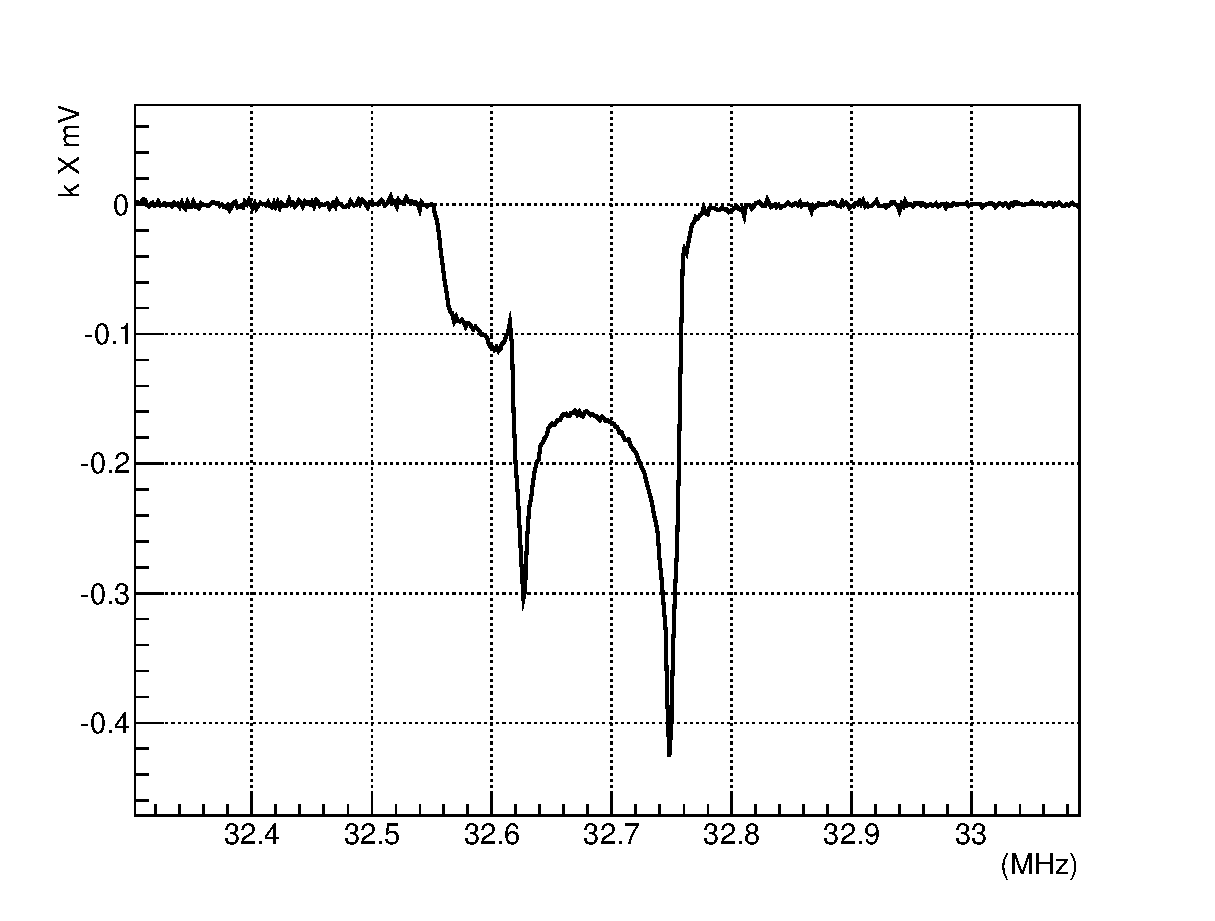
\includegraphics[width=3.0in,clip]{figs/study.eps}
\caption{The deuterium magnetic resonance line shape showing tensor polarization of more than 25\% after rf saturation of a pedestal.}  
\label{fig:study}
\end{figure}

\subsubsection{Depolarizing the Target}
%The NMR will be used on both to probe polarization.  
To move from polarized to unpolarized measurements, the target
polarization will be annihilated using destructive NMR loop field changes and destructive DNP microwave pumping.
It is also possible to remove LHe in the nose of the target to remove the polarization by heating.
During unpolarized data taking the incident electron beam heating is enough to remove the thermal equilibrium polarization.

The NMR measurement will ensure zero polarization.  The target material will be
kept at $\sim$1 K for polarized and unpolarized data collection, and the target field
will be held constant for both states as well.  These
consistencies are used to minimize the systematic differences in the
polarized and unpolarized data collection.  To minimize systematic effects over
time, the polarization condition will be switched twice in a 24 hour period. 
This is expected to account for drift in integrated charge accumulation.

%(I think we should move this discussion to another section dealing with target
%physics and the overhead time accounting. Also,  I would favor dumping the LHe, and refilling the
%nose.)}


\subsubsection{Rendering Dilution Factor}
\label{dil}
To derive the dilution factor, we first start with the ratio of 
polarized to unpolarized counts.
%equation used to obtain the observable in terms of each measured cross section.
%\begin{equation}
%\frac{A_{zz}P_{zz}}{2}=\left(\frac{\sigma^1-\sigma}{\sigma}\right).
%\end{equation}
In each case, the number of counts that are actually measured,  neglecting 
the small contributions of the thin aluminium cup window materials, NMR coils, etc.,
are
\begin{equation}
N_1=Q_1\varepsilon_1 {\cal A}_1 l_1[(\sigma_N+3\sigma_1)p_f+\sigma_{He}(1-p_f)],
\end{equation}
and
\begin{equation}
N=Q\varepsilon {\cal A}l[(\sigma_N+3\sigma)p_f+\sigma_{He}(1-p_f)].
\end{equation}
where $Q$ represents accumulated charge, $\varepsilon$ is the dectector 
efficiency, ${\cal A}$ the cup acceptance, and $l$ the cup length.  

For
this calculation we assume similar charge accumulation such that $Q\simeq Q_1$, 
and that the efficiencies stay constant, in which case all factors drop out of 
the ratio leading to
\begin{eqnarray}
\nonumber \frac{N_1}{N}& = &\frac{{(\sigma_N+3\sigma_1)p_f+\sigma_{He}(1-p_f)}
}{(\sigma_N+3\sigma)p_f+\sigma_{He}(1-p_f)}\\
\nonumber & = & \frac{{(\sigma_N+3\sigma(1+A_{zz}P_{zz}/2))p_f+\sigma_{He}(1-p_
f)}}{(\sigma_N+3\sigma)p_f+\sigma_{He}(1-p_f)}\\
\nonumber & = & \frac{{[(\sigma_N+3\sigma)p_f+\sigma_{He}(1-p_
f)]+3\sigma A_{zz}P_{zz}/2}}{(\sigma_N+3\sigma)p_f+\sigma_{He}(1-p_f)}\\
\nonumber & = & 1 + \frac{3\sigma 
A_{zz}P_{zz}/2}{(\sigma_N+3\sigma)p_f+\sigma_{He}(1-p_f)}\\
& = & 1 + \frac{1}{2} f A_{zz}P_{zz}, 
\end{eqnarray}
where $\sigma_1 = \sigma(1+A_{zz}P_{zz}/2)$ has ben substituted, per 
Eq.~\ref{eq:one}, with $P_B =0$. It can be seen that the above result 
corresponds to Eq.~\ref{3}.


\subsection{Overhead}

Table~\ref{OVERHEAD} summarizes the expected overhead, which sums to \overheaddays days.
%In order to calibrate the target polarimetry, elastic scattering measurements will be performed at %an
%incident energy of 2.2 GeV.
The dominant overhead comes from switching from the polarized to unpolarized state and vice versa, and target anneals.  The target will need to be annealed about every other day, and the material replaced once a week.
Measurements of the dilution from the unpolarized materials contained in the target, and of the packing fraction due to the granular composition of the target material will be performed with a carbon target.

%Configuration changes include rotation of the magnetic field of the target from parallel to perpendicular and vice versa.

\begin{table}
\begin{center}
  \begin{tabular}{lrrr} \hline\hline
 Overhead & Number&Time Per (hr)&(hr)\\
\hline
Polarization/depolarization & 30&       2.0&     60.0\\
Target anneal             &   13&       4.0&     52.0\\
Target T.E. measurement   &    5&       4.0&     20.0\\
%Beamline survey          &    2&       8.0&     16.0\\
Target material change    &    4&       4.0&     16.0\\
Packing Fraction/Dilution runs &    6&       1.0&      6.0\\
\hline
%Pass change              &    0&       4.0&       0.0\\
BCM calibration           &    8&       2.0&      16.0\\
Optics                    &    3&       4.0&      12.0\\
Linac change              &    1&       8.0&      8.0\\
Momentum/angle change     &    3&       2.0&       6.0\\
%Arc Energy Meas.          &    3&       2.0&       6.0\\
\hline
                          &     &          &        \overheaddays days  \\
\hline
 \end{tabular}
 \end{center}
  \caption{\label{OVERHEAD} Major contributions to the overhead.}
\end{table}


\section{Summary}

The ratio of the S- and D-wave state of the deuteron is not well constrained by current wavefunction models, which is particularly important in describing tensor-related effects such as short range correlations. Measuring the tensor asymmetry $A_{zz}$ by electron scattering off of tensor polarized deuterons in the quasi-elastic region region provides necessary information for extracting this ratio. With \productiondays days of beam and an additional \overheaddays days of overhead, $A_{zz}$ can be measured at $Q^2=1.5$, $0.7$, and $0.3~(\mathrm{GeV}/c)^2$ in Hall C using identical equipment as the upcoming $b_1$ measurement while being less sensitive to systematic uncertainties. In addition, it will fill a gap in measurements of $A_{zz}$ between the $T_{20}\propto A_{zz}$ elastic measurements and the $b_1\propto \frac{A_{zz}}{F_1^d}$ deep-inelastic measurements. 

% \section{Summary}

\clearpage
\appendix
%\section{Rates and Kinematics}
%\begin{figure}
%\begin{center}
%\includegraphics[width=1.0\textwidth,angle=00]{newfigs/ellie/b1_rates_hms_shms.eps}
%\caption{\label{PROJDETAIL}
%{\bf Top Left: }
%Projected precision of the tensor structure function $b_1$  with \production_days days of beam time.
%{\bf Right:}
%Corresponding projected precision of the tensor asymmetry $A_{zz}$.
%Data at different $Q^2$ are combined with an x-binning that varies slightly per point, but is approximately $\pm0.05$.
%%The black band
%%represents the systematic uncertainty.
%Also shown are the HERMES data~\cite{Airapetian:2005cb}, and the calculations from Kumano~\cite{Kumano:2010vz}, Miller~\cite{Miller:1989nc,Miller_tmp}, and Sargsian~\cite{MISAK}.
%}
%\end{center}
%\end{figure}

%\section{Statistical error calculations of $A_{zz}$}
%%\subsubsection{Statistical error calculations of $A_{zz}$ and $b_1^d$}
\label{APPERR}
Full details of the error calculation can be found in Ref.~\cite{SOLVI}.

From section 6 of Ref.~\cite{Hoodbhoy:1988am},
%Hoodbhoy, Jaffe and Manihar (Nuc. Phys. B312, p571-588, 1989), 
we have:


\begin{eqnarray}
\frac{d\sigma_{\parallel}^H}{dxdy} & = & K \Bigg[x F_1(x) + \Big(\frac{2}{3} - H^2\Big) x b_1(x) \Bigg]\\
\frac{d\sigma_{\perp}^H}{dxdy}    & = & K \Bigg[x F_1(x) - \Big(\frac{1}{3} - \frac{1}{2}H^2\Big) x b_1(x) \Bigg]
\label{xs} 
\end{eqnarray}
%
with $K = \frac{e^4 M E}{2 \pi Q^4} [1+(1-y)^2]$.
%
For simplicity, we use $\sigma_{\parallel}$ for $\frac{d\sigma_{\parallel}^H}{dxdy}$ and $\sigma_{\perp}$ for $\frac{d\sigma_{\perp}^H}{dxdy}$.

%From Jaffe's email, 
We know that $H^2 = (P_z+2)/3$, where $P_z$ is the vector polarization of the target. 
%This is where is my doubt. From the paper and Jaffe's email, they define $H$ as the polarization along the beam. So my understanding is that $P = P_z$ and it is the vector polarization. 
%
And the tensor polarization $P_{zz}$ is related to $P_z$ via Eq.~\ref{TENSORVECTOR}.
%\begin{eqnarray}
%P_{zz} = 2 - \sqrt{4 - 3 P_z^2}
%\label{none} 
%\end{eqnarray}

The tensor asymmetry $A_{zz}$ depends on $b_1$ and $F_1$:
\begin{eqnarray}
\frac{b_1}{F_1} = - \frac{3}{2} A_{zz}
\label{none} 
\end{eqnarray}


Working with the equations of $\sigma_{\parallel}$ and $\sigma_{\perp}$, we can isolate $A_{zz}$ to find: 
\begin{eqnarray}
\frac{\sigma_{\parallel} - \sigma_{\perp}}{\sigma_{\parallel} + 2 \sigma_{\perp}} = \frac{1}{4} P_z A_{zz}
\label{MAIN} 
\end{eqnarray}

Note, that if the vector polarization in the parallel orientation $P_z^\parallel$
differs from the polarization in the perpendicular orientation
$P_z^\perp$, then Eq.~\ref{MAIN} is modified slightly to:
\begin{eqnarray*}
\frac{\sigma_{\parallel} - \sigma_{\perp}}{\kappa\sigma_{\parallel} + 2 \sigma_{\perp}} = \frac{1}{4} P_z^\parallel A_{zz}
\end{eqnarray*}
where $\kappa={P_z^\perp}/{P_z^\parallel}$.   We've assumed $\kappa=1$ for rates calculations.



In order to calculate the statistical error on $A_{zz}$ we start from:
\begin{eqnarray}
(\delta A_{zz})^2 = \Bigg( \frac{\delta A_{zz}}{\delta \sigma_{\parallel}} \Bigg)^2 (\delta \sigma_{\parallel})^2 + \Bigg( \frac{\delta A_{zz}}{\delta \sigma_{\perp}} \Bigg)^2 (\delta \sigma_{\perp})^2
\label{none} 
\end{eqnarray}
and
\begin{eqnarray*}
\frac{\delta A_{zz}}{\delta \sigma_{\parallel}} & = &\frac{4}{P_z} \Bigg[\frac{- (\sigma_{\parallel} - \sigma_{\perp})}{(\sigma_{\parallel} + 2 \sigma_{\perp})^2} + \frac{1}{\sigma_{\parallel} + 2 \sigma_{\perp}} \Bigg] \\
         & = & \frac{4}{P_z} \frac{3 \sigma_{\perp}}{(\sigma_{\parallel} + 2 \sigma_{\perp})^2}
\label{none} 
\end{eqnarray*}


\begin{eqnarray*}
\frac{\delta A_{zz}}{\delta \sigma_{\perp}} & = &\frac{4}{P_z} \Bigg[\frac{- 2 (\sigma_{\parallel} - \sigma_{\perp})}{(\sigma_{\parallel} + 2 \sigma_{\perp})^2} - \frac{1}{\sigma_{\parallel} + 2 \sigma_{\perp}} \Bigg] \\
         & = & \frac{4}{P_z} \frac{-3 \sigma_{\parallel}}{(\sigma_{\parallel} + 2 \sigma_{\perp})^2}
\label{none} 
\end{eqnarray*}
%
to arrive at:
\begin{eqnarray}
(\delta A_{zz})^2 = \Bigg(\frac{4}{P_z}\Bigg)^2 \Bigg[ \frac{9 \sigma_{\perp}^2 \delta \sigma_{\parallel}^2 + 9\sigma_{\parallel}^2 \delta \sigma_{\perp}^2 }{(\sigma_{\parallel} + 2 \sigma_{\perp})^4} \Bigg]
\label{none} 
\end{eqnarray}

The parallel and perpendicular cross sections have the same kinematical weight $K$. Since $b_1$ is very small compared to $F_1$ (or equivalently, $A_{zz}$ is very small), we can make the assumption $\sigma_{\parallel} \approx \sigma_{\perp} \equiv \sigma$ and  $\delta \sigma_{\parallel} \approx  \delta \sigma_{\perp} \equiv \delta \sigma$. 

\begin{eqnarray}
(\delta A_{zz})^2 = \frac{9 \times 16}{P_z^2} \frac{2 \sigma^2 \delta \sigma^2}{(3 \sigma)^4} = \frac{32}{9 P_z^2} \frac{\delta \sigma^2}{\sigma^2}
\label{none} 
\end{eqnarray}

\begin{eqnarray}
\delta A_{zz} = \frac{4 \sqrt{2}}{3 P_z} \frac{\delta \sigma}{\sigma} =  \frac{4 \sqrt{2}}{3 P_z} \frac{1}{\sqrt{N}}
\label{none} 
\end{eqnarray}

We determine $N$ from the unpolarized cross section model~\cite{Martin:2009iq}, which then allows us to calculate the rates and the time.

\begin{eqnarray}
N = \frac{32}{9} \frac{1}{P_z^2 (\delta A_{zz}^{meas})^2}
\label{none} 
\end{eqnarray}

To get the rates as a function of the theoretical tensor asymmetry, we need to apply the dilution factors:
\begin{eqnarray}
A_{zz}^{meas} = f P_{zz} A_{zz}
\label{none} 
\end{eqnarray}

\begin{eqnarray}
N = \frac{32}{9} \frac{1}{P_z^2 (f P_{zz} \delta A_{zz})^2}
\label{none} 
\end{eqnarray}

We need $N/2$ events in parallel and perpendicular kinematics. If we had a pure deuterium target, the time need will be:
\begin{eqnarray}
T = \frac{N}{R_D} = \frac{32}{9} \frac{1}{R_D P_z^2 (f P_{zz} \delta A_{zz})^2}
\label{none} 
\end{eqnarray}

Now the deuterium rates are estimated from the unpolarized deuteron cross section model~\cite{Martin:2009iq} $\sigma_D$:
\begin{eqnarray}
 R_D = \sigma_D~dp~d\Omega~L = \sigma_D~dp~d\Omega~\rho_D~\frac{I}{e}
\label{none} 
\end{eqnarray}
%
with $\rho_D = \rho_{LiD} \cdot f_{LiD} \cdot PF_{LiD}$, where $f_{LiD}$ is the dilution and $PF_{LiD}$ is the packing fraction.





%\label{APPERR}
Full details of the error calculation can be found in Ref.~\cite{SOLVI}.
%
From section 6 of Ref.~\cite{Hoodbhoy:1988am},
%Hoodbhoy, Jaffe and Manihar (Nuc. Phys. B312, p571-588, 1989),
we have:

\begin{eqnarray}
\frac{d\sigma_{\parallel}^H}{dxdy} & = & K \Bigg[x F_1(x) + \Big(\frac{2}{3} - H^2\Big) x b_1(x) \Bigg]\\
\frac{d\sigma_{\perp}^H}{dxdy}    & = & K \Bigg[x F_1(x) - \Big(\frac{1}{3} - \frac{1}{2}H^2\Big) x b_1(x) \Bigg]
\label{xs} 
\end{eqnarray}
%
with $K = \frac{e^4 M E}{2 \pi Q^4} [1+(1-y)^2]$.

For simplicity, we will use $\sigma_{\parallel}$ for $\frac{d\sigma_{\parallel}^H}{dxdy}$ and $\sigma_{\perp}$ for $\frac{d\sigma_{\perp}^H}{dxdy}$.


We know that $H^2 = (P+2)/3$, where $P$ is the vector polarization of the target. 
And the tensor polarization $P_{zz}$ is related to $P_z$ via Eq.~\ref{TENSORVECTOR}.

The tensor asymmetry $A_{zz}$ depends on $b_1$ and $F_1$:
\begin{eqnarray}
\frac{b_1}{F_1} = - \frac{3}{2} A_{zz}
\label{none} 
\end{eqnarray}

\subsection{Cross section method}

Working with the equations of $\sigma_{\parallel}$ and $\sigma_{\perp}$, we can isolate $b_{1}$:

\begin{eqnarray}
\sigma_{\parallel} - \sigma_{\perp} = \frac{-K}{6} (2 P_z^{\parallel} + P_z^{\perp}) x b_1
\label{MAIN}
\end{eqnarray}
where $P_z^{\parallel}$ and $P_z^{\perp}$ are the vector polarization achieved in the longitudinal and transverse configurations respectively.
%
%Note, that if the vector polarization in the parallel orientation $P_z^\parallel$
%differs from the polarization in the perpendicular orientation
%$P_z^\perp$, then Eq.~\ref{MAIN} is modified slightly to:
%\begin{eqnarray*}
%\frac{\sigma_{\parallel} - \sigma_{\perp}}{\kappa\sigma_{\parallel} + 2 \sigma_{\perp}} = \frac{1}{4} P_z^\parallel A_{zz}
%\end{eqnarray*}
%where $\kappa={P_z^\perp}/{P_z^\parallel}$.   We've assumed $\kappa=1$ for rates calculations.

\begin{eqnarray}
\frac{\delta b_1}{b_1} = \frac{\sqrt{\delta \sigma_{\perp}^2 + \delta \sigma_{\parallel}^2}}{\sigma_{\perp} - \sigma_{\parallel}} 
\label{none} 
\end{eqnarray}

In the valence region, $b_1 < 0$ which implies $\sigma_{\perp} < \sigma_{\parallel}$. We can define the difference between $\sigma_{\perp}$ and $\sigma_{\parallel}$ as:

\begin{eqnarray}
\sigma_{\parallel} = (1+\epsilon) \sigma_{\perp}
\label{none} 
\end{eqnarray}

It is safe to assume that we will need $\delta \sigma_{\perp} \approx \delta \sigma_{\parallel}$. We obtain:
\begin{eqnarray}
\frac{\delta b_1}{b_1} = - \frac{\sqrt{2}}{\epsilon} \frac{\delta \sigma_{\perp}}{\sigma_{\perp}} 
\label{none} 
\end{eqnarray}

Now to evaluate the time necessary to perform a significant measurement of $b_1$, we need an estimate of the value of $\epsilon$.  So we start from:
\begin{eqnarray}
\sigma_{\parallel} & = & \sigma_{u} (1 - \frac{1}{3} P_z^{\parallel} \frac{b_1}{F_1}) \\
\sigma_{\perp} & = & \sigma_{u} (1 + \frac{1}{6} P_z^{\perp} \frac{b_1}{F_1})
\label{none} 
\end{eqnarray}
%
with $\sigma_u$ the unpolarized cross section.  Which leads to:

\begin{eqnarray}
\epsilon = & \frac{1 - \frac{1}{3} P_z^{\parallel} \frac{b_1}{F_1}}{1 + \frac{1}{6} P_z^{\perp} \frac{b_1}{F_1}}
\label{EPSILON} 
\end{eqnarray}

We use for $b_1^d$ the fit from Kumano~\cite{Kumano:2010vz} and for $F_1^d$ MSTW~\cite{Martin:2009iq} (no EMC effect or smearing included). For $x$-values of 0.30, 0.40 and 0.50, $\epsilon$ is equal to 0.0013, 0.0026 and 0.0037 respectively, assuming $P_z^{\perp} = P_z^{\parallel} = 0.35$

\begin{eqnarray}
\frac{\delta b_1}{b_1} = - \frac{\sqrt{2}}{\epsilon} \frac{1}{\sqrt{N}} 
\label{none} 
\end{eqnarray}

The number of events needed in each parallel and perpendicular kinematics are $N/2$ with:
\begin{eqnarray}
N = \frac{2}{\epsilon^2} \frac{1}{(\delta b_1 / b_1)^2}
\label{none} 
\end{eqnarray}

The time necessary to achieve this statistics is:
\begin{eqnarray}
T = \frac{N}{R_D} = \frac{2}{\epsilon^2 R_D (\delta b_1 / b_1)^2}
\label{none} 
\end{eqnarray}

The deuterium rates are estimated from the unpolarized deuteron cross section~\cite{Martin:2009iq} $\sigma_D$:
%MRST2008:
\begin{eqnarray}
 R_D = \sigma_D~dp~d\Omega~L = \sigma_D~dp~d\Omega~\rho_D~\frac{I}{e}
\label{none} 
\end{eqnarray}
%
with $\rho_D = \rho_{ND3} \cdot f_{ND3} \cdot PF_{ND3}$, where $f_{ND3}$ is the dilution and $PF_{ND3}$ is the packing fraction. To estimate the physics rates, the spectrometer acceptance and momentum bite were reduced to $d\Omega = 6.5$ msr and $dp = \pm$8\% for the HMS and $d\Omega = 4.4$ msr and $dp = ^{+20\%} _{-8\%}$ for SHMS and a cut on $W \ge 1.8$ GeV was required.



%%\section{Asymmetry method}
%
%Working with the equations of $\sigma_{\parallel}$ and $\sigma_{\perp}$, we can isolate $A_{zz}$:
%\begin{eqnarray}
%\frac{\sigma_{\parallel} - \sigma_{\perp}}{\sigma_{\parallel} + 2 \sigma_{\perp}} = \frac{1}{4} P_z A_{zz}
%\label{none} 
%\end{eqnarray}
%
%\vspace{0.5cm}
%\underline{Calculation of $A_{zz}$ statistical error}
%\begin{eqnarray}
%(\delta A_{zz})^2 = \Bigg( \frac{\delta A_{zz}}{\delta \sigma_{\parallel}} \Bigg)^2 (\delta \sigma_{\parallel})^2 + \Bigg( \frac{\delta A_{zz}}{\delta \sigma_{\perp}} \Bigg)^2 (\delta \sigma_{\perp})^2
%\label{none} 
%\end{eqnarray}
%
%\begin{eqnarray}
%\frac{\delta A_{zz}}{\delta \sigma_{\parallel}} & = &\frac{4}{P_z} \Bigg[\frac{- (\sigma_{\parallel} - \sigma_{\perp})}{(\sigma_{\parallel} + 2 \sigma_{\perp})^2} + \frac{1}{\sigma_{\parallel} + 2 \sigma_{\perp}} \Bigg] \\
%         & = & \frac{4}{P_z} \frac{3 \sigma_{\perp}}{(\sigma_{\parallel} + 2 \sigma_{\perp})^2}
%\label{none} 
%\end{eqnarray}
%
%
%\begin{eqnarray}
%\frac{\delta A_{zz}}{\delta \sigma_{\perp}} & = &\frac{4}{P_z} \Bigg[\frac{- 2 (\sigma_{\parallel} - \sigma_{\perp})}{(\sigma_{\parallel} + 2 \sigma_{\perp})^2} - \frac{1}{\sigma_{\parallel} + 2 \sigma_{\perp}} \Bigg] \\
%         & = & \frac{4}{P_z} \frac{-3 \sigma_{\parallel}}{(\sigma_{\parallel} + 2 \sigma_{\perp})^2}
%\label{none} 
%\end{eqnarray}
%
%\begin{eqnarray}
%(\delta A_{zz})^2 = \Bigg(\frac{4}{P_z}\Bigg)^2 \Bigg[ \frac{9 \sigma_{\perp}^2 \delta \sigma_{\parallel}^2 + 9\sigma_{\parallel}^2 \delta \sigma_{\perp}^2 }{(\sigma_{\parallel} + 2 \sigma_{\perp})^4} \Bigg]
%\label{none} 
%\end{eqnarray}
%
%The parallel and perpendicular cross sections have the same kinematical weight $K$. Since $b_1$ is very small compared to $F_1$ (or $A_{zz}$ is very small), we can make the assumption $\sigma_{\parallel} \approx \sigma_{\perp} \equiv \sigma$ and  $\delta \sigma_{\parallel} \approx  \delta \sigma_{\perp} \equiv \delta \sigma$. 
%
%\begin{eqnarray}
%(\delta A_{zz})^2 = \frac{9 \times 16}{P_z^2} \frac{2 \sigma^2 \delta \sigma^2}{(3 \sigma)^4} = \frac{32}{9 P_z^2} \frac{\delta \sigma^2}{\sigma^2}
%\label{none} 
%\end{eqnarray}
%
%\begin{eqnarray}
%\delta A_{zz} = \frac{4 \sqrt{2}}{3 P_z} \frac{\delta \sigma}{\sigma} =  \frac{4 \sqrt{2}}{3 P_z} \frac{1}{\sqrt{N}}
%\label{none} 
%\end{eqnarray}
%
%I get $N$ from the unpolarized cross sections. Then I calculate the rates and the time.
%
%\begin{eqnarray}
%N = \frac{32}{9} \frac{1}{P_z^2 (\delta A_{zz}^{meas})^2}
%\label{none} 
%\end{eqnarray}
%
%To get the rates as a function of the theoretical tensor asymmetry, we need to apply the dilution factors:
%\begin{eqnarray}
%A_{zz}^{meas} = f P_{zz} A_{zz}
%\label{none} 
%\end{eqnarray}
%
%\begin{eqnarray}
%N = \frac{32}{9} \frac{1}{P_z^2 (f P_{zz} \delta A_{zz})^2}
%\label{none} 
%\end{eqnarray}
%
%We need $N/2$ events in parallel and perpendicular kinematics. If I had a pure deuterium target, the time need will be:
%\begin{eqnarray}
%T = \frac{N}{R_D} = \frac{32}{9} \frac{1}{R_D P_z^2 (f P_{zz} \delta A_{zz})^2}
%\label{none} 
%\end{eqnarray}
%
%Now the deuterium rates are estimated from the unpolarized deuteron cross section $\sigma_D$:
%\begin{eqnarray}
% R_D = \sigma_D~dp~d\Omega~L = \sigma_D~dp~d\Omega~\rho_D~\frac{I}{e}
%\label{none} 
%\end{eqnarray}
%
%with $\rho_D = \rho_{LiD} \cdot f_{LiD} \cdot PF_{LiD}$, where $f_{LiD}$ is the dilution and $PF_{LiD}$ is the packing fraction.
%
%
%
%

%%\section{Statistical Uncertainty Calculation}
\label{stat}
To investigate the statistical uncertainty we start with the equation for $A_{zz}$ using
measured counts for polarized data $N_1$ and unpolarized data $N$, 
\begin{equation}
A_{zz}=\frac{2}{fP_{zz}}\left(\frac{N_1-N}{N}\right).
\end{equation}
The absolute error with respect to counts in then,
\begin{equation}
\delta A_{zz}=\frac{2}{fP_{zz}}\sqrt{\left(\frac{\delta N_1}{N}\right)^2+\left(\frac{N_1\delta N}{N^2}\right)^2}.
\end{equation}
To approximate, assume $N_1\simeq N$, so that twice $N$ is required to obtain the total number of count
$N_T$ for the experiment leading to,
\begin{equation}
\delta A_{zz}=\frac{4}{fP_{zz}}\frac{1}{\sqrt{N_T}}.
\end{equation}



%  Go to fullpage mode

\topmargin 0pt
\advance \topmargin by -\headheight
\advance \topmargin by -\headsep

\textheight 8.9in

\oddsidemargin 0pt
\evensidemargin \oddsidemargin
\marginparwidth 0.5in

\textwidth 6.5in
\clearpage
%\begin{thebibliography}{99}
%\input{input/bib.tex}
%\end{thebibliography}

\bibliography{input/bibliography}
\end{document}
